\documentclass[conference]{IEEEtran}
\IEEEoverridecommandlockouts
% The preceding line is only needed to identify funding in the first footnote. If that is unneeded, please comment it out.
\usepackage{cite}
\usepackage{amsmath,amssymb,amsfonts}
\usepackage{algorithmic}
\usepackage{graphicx}
\usepackage{textcomp}
\usepackage{xcolor}
\usepackage{hyperref}
\def\BibTeX{{\rm B\kern-.05em{\sc i\kern-.025em b}\kern-.08em
    T\kern-.1667em\lower.7ex\hbox{E}\kern-.125emX}}
\begin{document}

\title{Design, Implementation, and Analysis of an AM Modulator and Demodulator\\
{\Large Electronic Workshop 2 - Project 2}
}


\author{\IEEEauthorblockN{\textbf{Chamarthy Madhan Sai Krishna}}
\IEEEauthorblockA{\textit{Electronics \& Communication Engineering} \\
\textit{IIIT Hyderabad}\\
chamarthymadhan.k@students.iiit.ac.in\\2023102030}
\and
\IEEEauthorblockN{\textbf{Sajiv Singh}}
\IEEEauthorblockA{\textit{Electronics \& Communication Engineering} \\
\textit{IIIT Hyderabad}\\
sajiv.singh@research.iiit.ac.in\\2023112003}
}
\maketitle

\begin{abstract}

The project focuses on the design, implementation and analysis of a Double Sideband Suppressed Carrier (DSB-SC) Amplitude Modulation(AM) modulator and demodulator circuit prototype.

The main goal was to modulate the carrier signal, generated by the Local Oscillator (LO), using the modulating signal from the DSO, and to successfully recover the original signal.

Through practical implementation, the project demonstrates the fundamental concepts of Communication Theory. The circuit helps in understanding how information can be encoded and transmitted over a carrier signal using AM techniques.
\end{abstract}

% \begin{IEEEkeywords}
% component, formatting, style, styling, insert
% \end{IEEEkeywords}

\section{To-do: }
\begin{itemize}
    \item Improvise the photos of the spectrums - conventional AM and DSB-SC AM
    \item add github link, youtube video link
    \item add calculations, simulations, outputs, 
    
\end{itemize}

\section{Introduction}

\subsection{Background of Amplitude Modulation}
Amplitude Modulation (AM) is a modulation technique where the amplitude (signal strength) of a carrier wave is varied in proportion to the message signal (e.g., audio). It's commonly used in electronic communication for transmitting messages via radio waves.
In AM,  carrier signal's amplitude, A(t), changes according to the message signal.  This message signal defines the envelope of the transmitted waveform. In the frequency domain, AM produces a signal with power concentrated at the carrier frequency and two adjacent sidebands.

\textit{Types of Amplitude Modulation: }
\begin{itemize}
    \item \textit{Double-Sideband Amplitude Modulation (DSB-AM): } The standard AM method generates sidebands on both sides of the carrier frequency. These sidebands contain the frequency components of the modulating signal and are symmetrically placed around the carrier frequency.
    \item \textit{Single-Sideband Modulation (SSB):} Uses bandpass filters to eliminate one sideband and possibly the carrier, improving power efficiency and bandwidth utilization.
    \item \textit{Quadrature Amplitude Modulation (QAM): }A more complex form of Amplitude modulation is often used with digital data to enable more efficient use of bandwidth.
    \item \textit{ Double-Sideband Suppressed Carrier (DSB-SC): } This technique removes the carrier signal, transmitting only the upper and lower sidebands. It improves power efficiency but requires coherent detection at the receiver.
    \item \textit{Vestigial Sideband Modulation (VSB): } VSB retains part of one sideband while suppressing the rest of the unwanted sideband. This method helps reduce the bandwidth required for transmission, offering a more efficient use of spectrum compared to standard AM, while still allowing for accurate signal recovery at the receiver.
    \item \textit{Pulse Amplitude Modulation (PAM): }PAM varies the amplitude of pulses rather than a continuous wave. It is used in digital communication systems as an intermediate step before converting signals to binary formats.
\end{itemize}


\subsection{Objectives}
Following are the primary objectives of this project: 
\begin{enumerate}
    \item To design and implement a Double Sideband Suppressed Carrier (DSB-SC) Amplitude Modulation (AM) modulator circuit capable of encoding a modulating signal onto a carrier signal generated by a Local Oscillator (LO).
    \item To design and implement a corresponding demodulator circuit that can successfully recover the original modulating signal from the received DSB-SC AM signal.
    \item To analyze the performance of the implemented modulator and demodulator circuits through practical experimentation, demonstrating the principles of amplitude modulation in communication systems.
    
\end{enumerate}

% \subsection{}

\section{Theoretical Background of AM}
% In conventional AM, a message signal $m(t)$ modulates the amplitude of a high frequency carrier wave $c(t) = A_c cos(2\pi f_ct)$. The modulated signal becomes
% \[
% S_{AM}(t) = A_c [1 + \mu_am(t)]cos(2 \pi f_c t) 
% \] 
% where $\mu_a$ is the modulation index. This creates two sidebands and a dominant carrier component in the frequency spectrum.Double Sideband Suppresed Carrier (DSB-SC) improves power efficiency by eliminating the carrier component:
% \[
% S_{DSB}(t) = A_cm(t)cos(2 \pi f_c t) 
% \]

% This results in two mirrored sidebands in the frequency spectrum, both carrying identical information, and the absence of a carrier component. The Fourier transform reveals:
% \[
% S_{DSB}(\omega) = \frac{A_c}{2} \left[ M(\omega - \omega_c) + M(\omega + \omega_c) \right]
% \]

\textbf{\textit{Modulation: }}
In conventional AM, we add a large carrier component to a DSB-SC signal, so that the passband transmitted signal is of the form: 
\[ u_{AM}(t) = A m(t) \cos(2\pi f_c t) + A_c \cos(2\pi f_c t) \]

Taking the Fourier transform, we have 
\[ U_{AM}(f) = \frac{A}{2} \left( M(f - f_c) + M(f + f_c) \right) +\]
\[ \frac{A_c}{2} \left( \delta(f - f_c) + \delta(f + f_c) \right) \]

which means that, in addition to the USB and LSB due to the message modulation, we also have impulses at \( \pm f_c \) due to the unmodulated carrier.

\begin{figure}
    \centering
    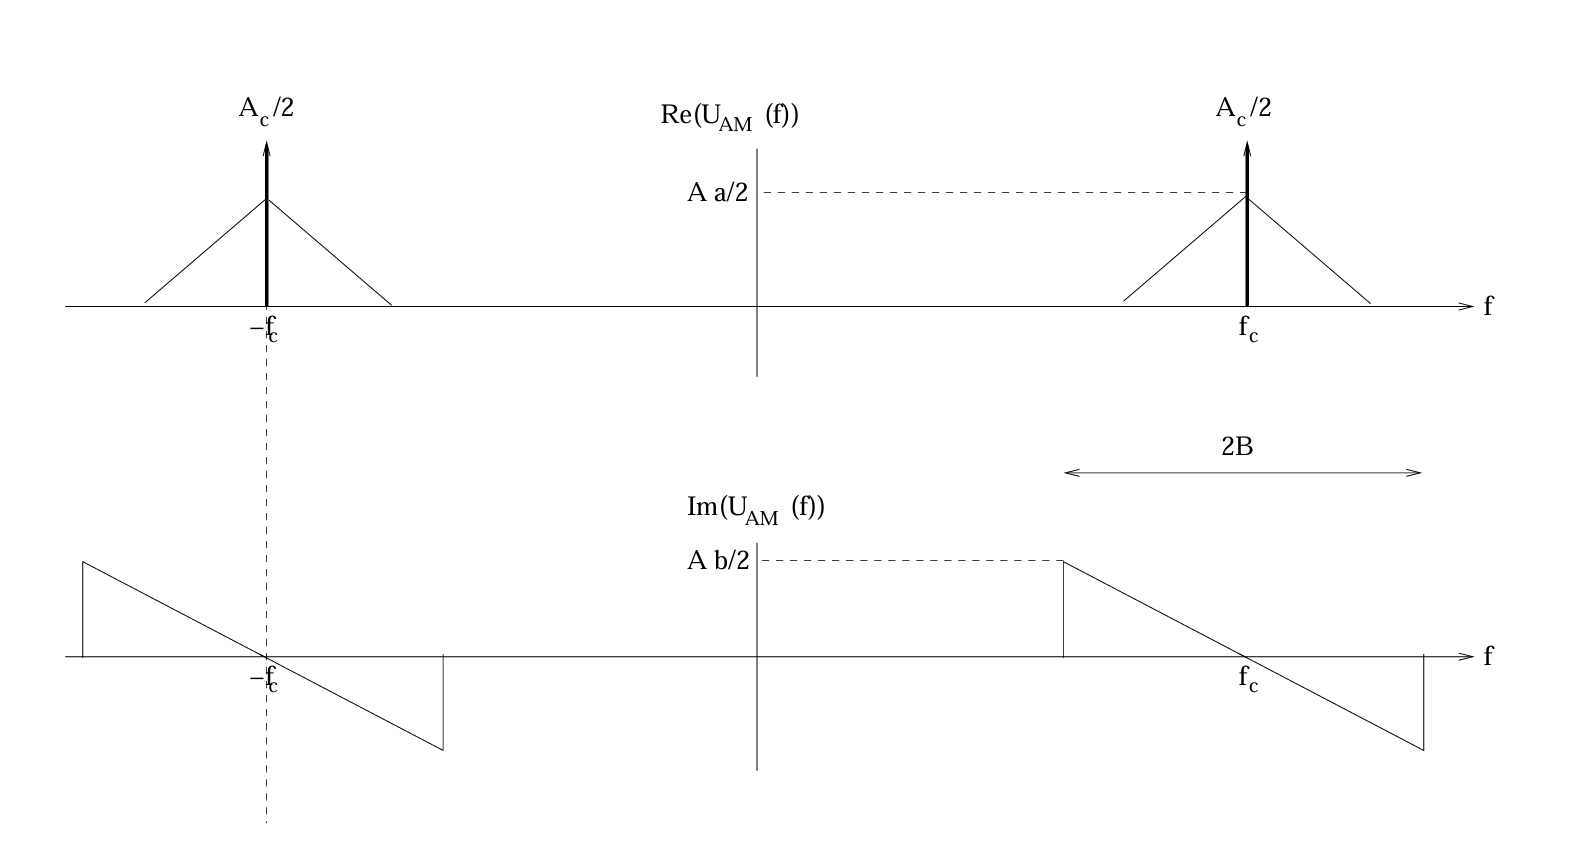
\includegraphics[width=1\linewidth]{Conventional_AM_spectrum.png}
    \caption{Spectrum of Conventional AM}
    % \label{fig:enter-label}
\end{figure}

The key concept behind conventional AM is that, by making \( A_c \) large enough, the message can be demodulated using a simple envelope detector. Large \( A_c \) corresponds to expending transmitter power on sending an unmodulated carrier which carries no message information, in order to simplify the receiver. This tradeoff makes sense in a broadcast context, where one powerful transmitter may be sending information to a large number of low-cost receivers, and is the design approach that has been adopted for broadcast AM radio. 

The key issue with conventional AM is its inefficiency in terms of power utilization. This led to the development of DSB-SC modulation which addresses these issues by suppressing the carrier and improving the power efficiency. 

  \[  u_{DSB}(t) = A m(t) \cos(2\pi f_c t) \]


Taking Fourier transforms, we have

   \[ U_{DSB}(f) = \frac{A}{2} \left( M(f - f_c) + M(f + f_c) \right) \]

   \begin{figure}
       \centering
       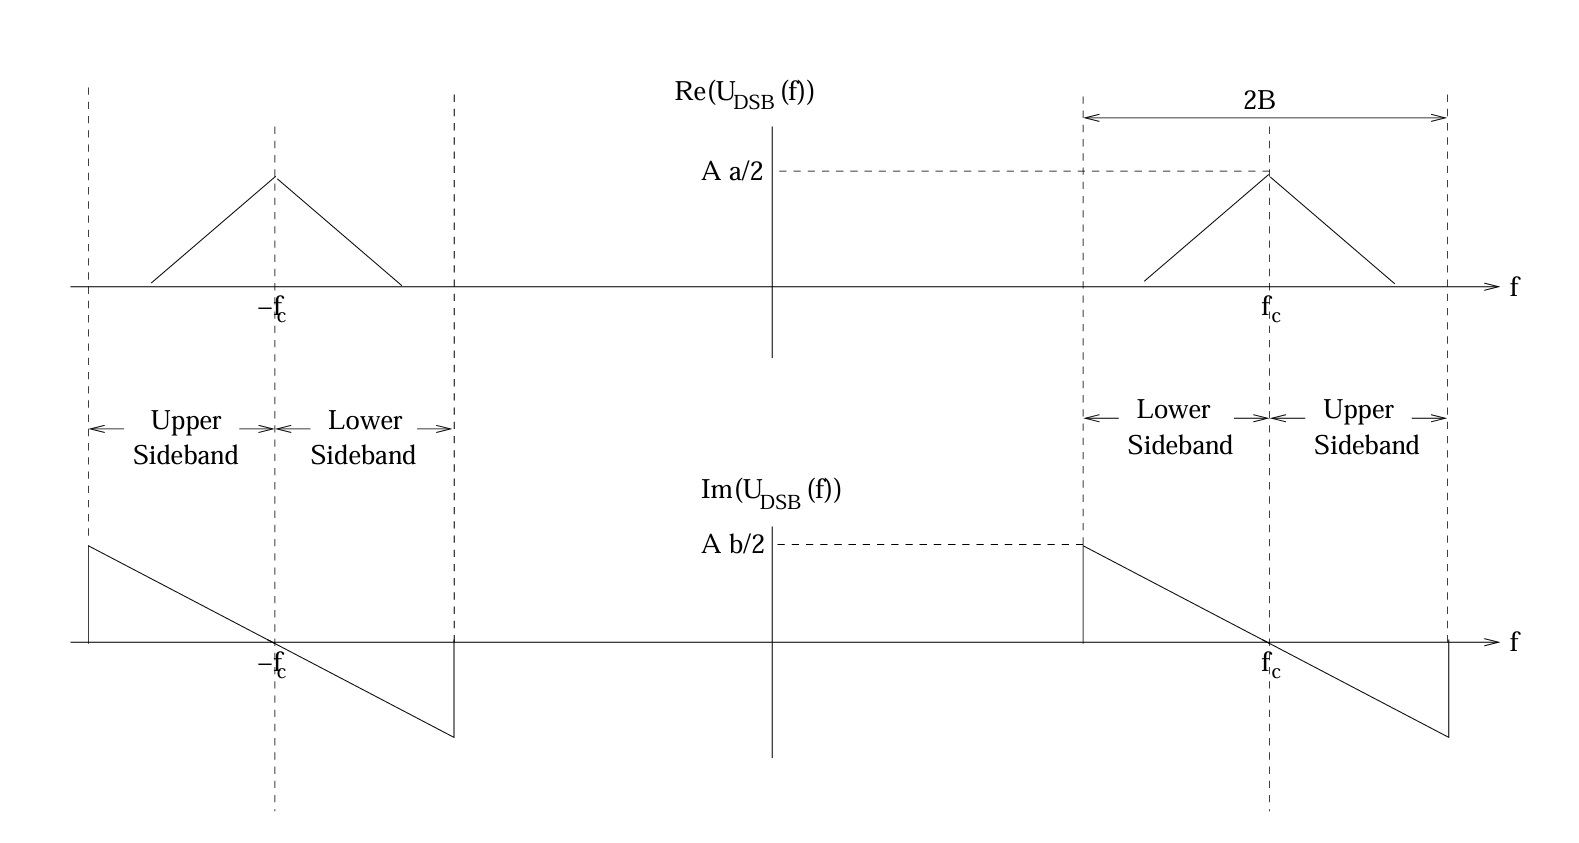
\includegraphics[width=1\linewidth]{DSB_SC_Passband_Spectrum.png}
       \caption{Spectrum of DSB-SC AM}
       % \label{fig:enter-label}
   \end{figure}

\textbf{\textit{Demodulation: }}
\begin{figure}
    \centering
    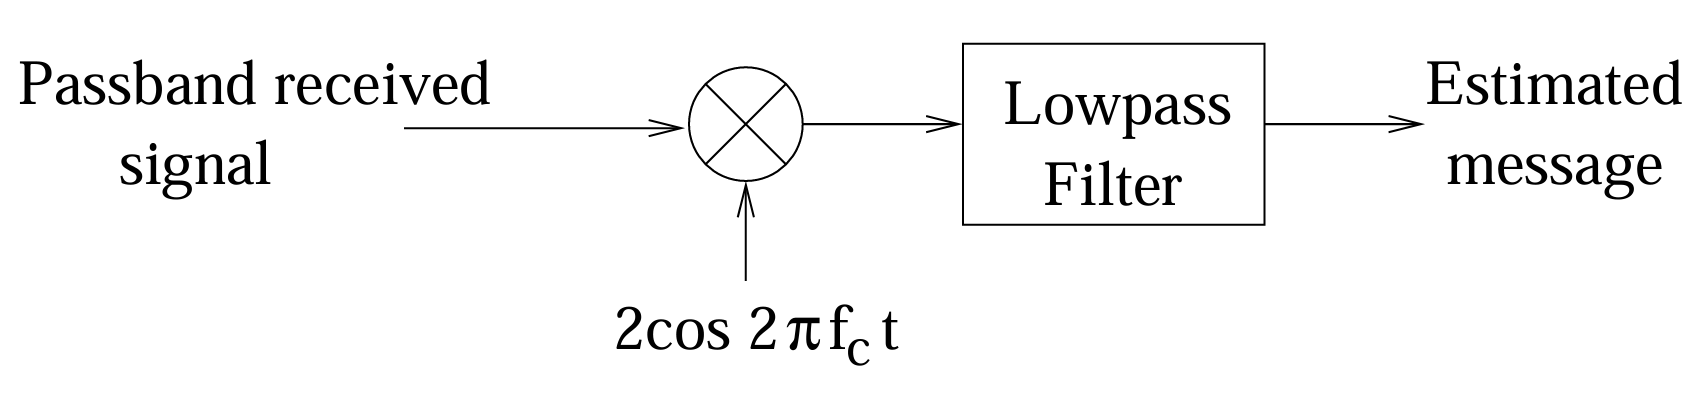
\includegraphics[width=1\linewidth]{Coherent_demodulation_AM.png}
    \caption{Coherent Demodulation of AM}
    % \label{fig:enter-label}
\end{figure}

Multiply the received signal with the cosine of the carrier, and pass it through a low-pass filter. Ignoring noise, the received signal is given by
\[
    y_p(t) = A m(t) \cos(2\pi f_c t + \theta_r)
\]

where \(\theta_r\) is the phase of the received carrier relative to the local copy of the carrier produced by the receiver’s local oscillator (LO), and \(A\) is the received amplitude, taking into account the propagation channel from the transmitter to the receiver. In order for this demodulator to work well, we must have \(\theta_r\) as close to zero as possible; that is, the carrier produced by the LO must be coherent with the received carrier.

The effect of phase mismatch:
\[
    2y_p(t) \cos(2\pi f_c t) = A m(t) \cos(2\pi f_c t + \theta_r) \cos(2\pi f_c t)
\]

\[
=A m(t) \cos\theta_r + A m(t) \cos(4\pi f_c t + \theta_r)
\]

We recognize the second term on the right-hand side as being a passband signal at \(2f_c\) (since it is a baseband message multiplied by a carrier whose frequency exceeds the message bandwidth). It is therefore rejected by the low-pass filter. The first term is a baseband signal proportional to the message, which appears unchanged at the output of the LPF (except possibly for scaling), as long as the LPF response has been designed to be flat over the message bandwidth. The output of the demodulator is therefore given by
\[
    \hat{m}(t) = A m(t) \cos\theta_r 
\]

The demodulator output is proportional to the message, which is what we want, but the proportionality constant varies with the phase of the received carrier relative to the LO. In particular, the signal gets significantly attenuated as the phase mismatch increases, and gets completely wiped out for \(\theta_r = \frac{\pi}{2}\).

Note that, if the carrier frequency of the LO is not synchronized with that of the received carrier (say with frequency offset \(\Delta f\)), then \(\theta_r(t) = 2\pi \Delta f t + \phi\) is a time-varying phase that takes all values in \([0, 2\pi)\), which leads to time-varying signal degradation in amplitude, as well as unwanted sign changes. Thus, for coherent demodulation to be successful, we must drive \(\Delta f\) to zero, and make \(\phi\) as small as possible; that is, we must synchronize to the received carrier.


\section{Circuit Design \& Implementation}
\subsection{Local Oscillator}
To generate the carrier signal (both at the transmitter end and the Local Oscillator (LO) signal for coherent demodulation at the receiver end), we have used a Wein Bridge Oscillator. The Wein Bridge Oscillator is a type of electronic oscillator that generates sine waves. It is based on the principle of positive and negative feedback, using a bridge circuit with resistors and capacitors to determine the frequency of oscillation. The circuit is known for its simplicity and ability to produce low-distortion sine waves.

\begin{figure}
    \centering
    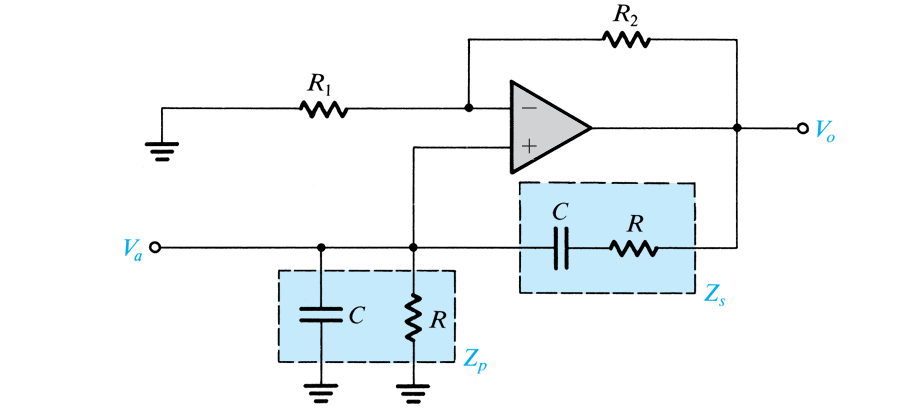
\includegraphics[width=1 \linewidth]{Images/Wein_bridge_osc_without_amp_stabilization.png}
    \caption{Circuit diagram of the Wein Bridge Oscillator}
    % \label{fig:enter-label}
\end{figure}

\begin{align}
    L(s) &= \left( 1 + \frac{R_2}{R_1} \right) 
            \cdot \frac{Z_p}{Z_p + Z_s} \nonumber \\
         &= \frac{1 + \tfrac{R_2}{R_1}}{1 + Z_s Y_p} \nonumber \\
         &= \frac{1 + \tfrac{R_2}{R_1}}{3 + sCR + \tfrac{1}{sCR}} \tag{17.10} \\
    %
    L(j\omega) &= \frac{1 + \tfrac{R_2}{R_1}}
                      {3 + j\left( \omega CR - \tfrac{1}{\omega CR} \right)} \tag{17.11} \\
    %
    \intertext{For zero phase (i.e., real loop gain):}
    \omega_0 CR &= \frac{1}{\omega_0 CR} \nonumber \\
    \Rightarrow \quad \omega_0 &= \frac{1}{CR} \tag{17.12} \\
    %
    \intertext{Barkhausen Criterion requires:}
    |L(j\omega_0)| &= 1 \quad \text{and} \quad 
    \angle L(j\omega_0) = 2n\pi \\
    %
    \intertext{To satisfy this, the gain condition is:}
    \frac{R_2}{R_1} &> 2 \nonumber
    \end{align}
    
    
    
The amplitude of oscillation can be determined and stabilized by using a nonlinear con
trol network. The below circuit is the Wein Bridge Oscillator with amplitude stabilization. The circuit uses the popular limiter circuit using diodes for amplitude control. 

\begin{figure}
    \centering
    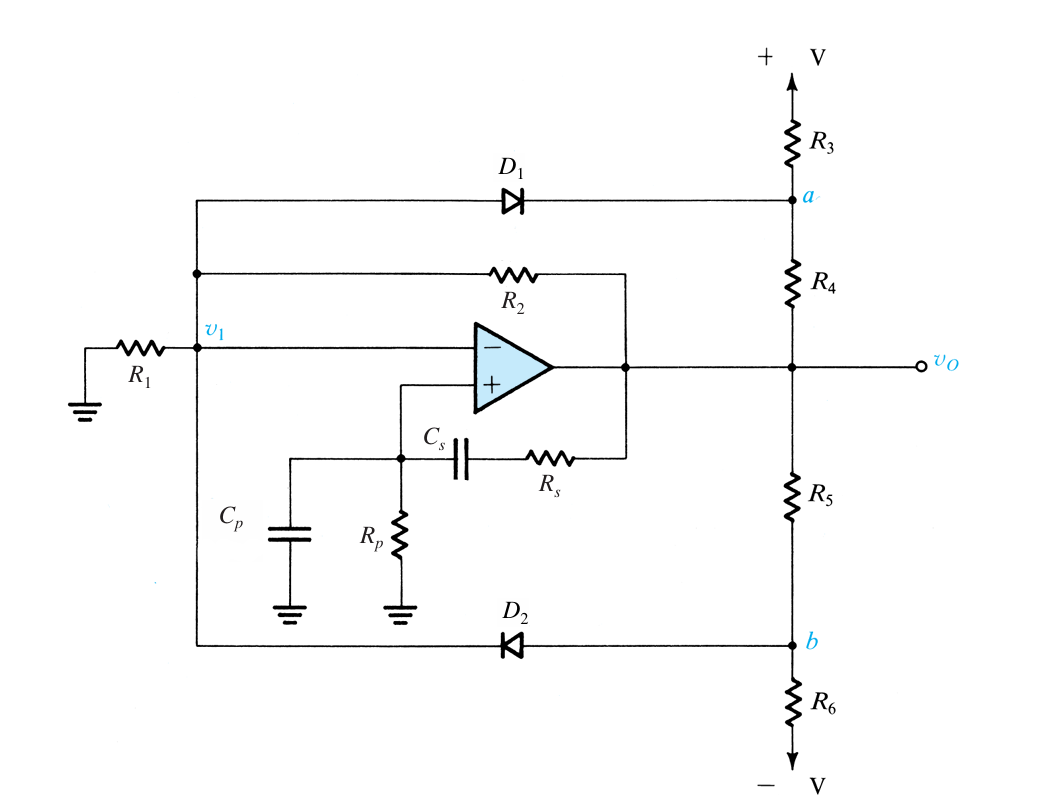
\includegraphics[width=1\linewidth]{Images/wein_bridge_osc_with_amp_stabilization.png}
    \caption{Circuit diagram of the Wein Bridge Oscillator with amplitude stabilization}
    % \label{fig:enter-label}
\end{figure}


\subsection{Modulator}
To perform modulation in our circuit, we have chosen to implement a switching mode modulator using a MOSFET as a switch. These kind of mixer circuits have high efficiency because a square wave is generated by turning the circuit on and off. When the circuit is off, no power is consumed. This circuit provides more linearity compared to non-linear mixers with a simpler design.
\begin{figure}
    \centering
    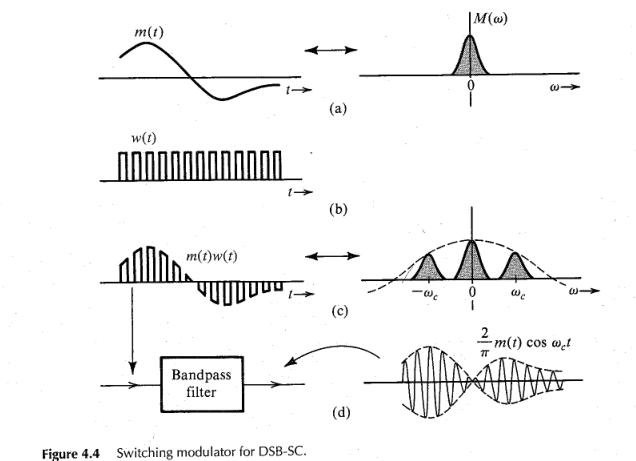
\includegraphics[width=0.85\linewidth]{Images/Switching_Modulator_Working.png}
    \caption{Working of the Switching Modulator Used in the Project}
    % \label{fig:enter-label}
\end{figure}

To make this switching modulator in LTSpice, we have used a npn MOSFET. The circuit is designed to modulate the message signal with the carrier signal. The message signal is fed into the gate of the MOSFET, while the carrier signal is fed into the drain. The output is taken from the source of the MOSFET. The circuit is designed to work in a switching mode, where the MOSFET operates as a switch (Voltage controlled resistor), turning on and off based on the input signals.

\begin{figure}
    \centering
    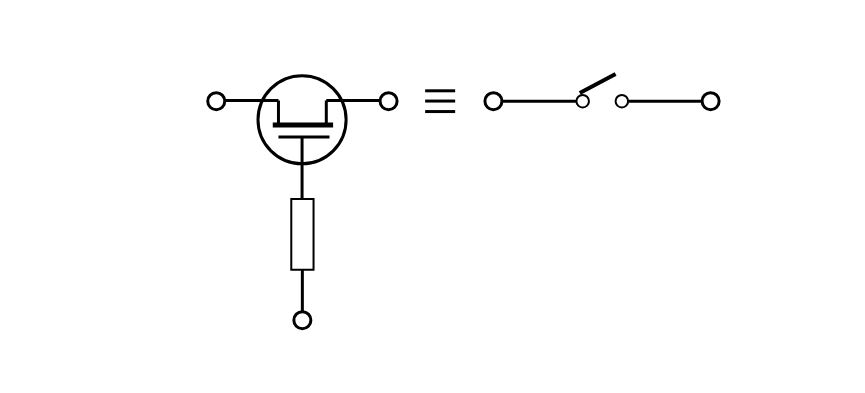
\includegraphics[width=1\linewidth]{Images/FET_mixer.png}
    \caption{FET as a Mixer}
    % \label{fig:enter-label}
\end{figure}


Considering m(t) as the message signal and f(t) as the carrier signal. For the given design to work as a mixer, it is really important to set the DC bias of the npn MOSFET used to its threshold. When the carrier wave (sinusoid produced by the oscillator) is added to this bias, then the MOSFET turns on in the positive cycle and turns off during the negative cycle. This happens because the operating point is set at $V_{TH}$. This effectively multiplies our message signal with a square wave of the frequency of our carrier. Let this square wave be denoted by w(t). A a square wave is a periodic wave with a valid Fourier series expression. The Fourier series representation of w(t) and the result of the multiplication is given by:
$$w(t) = \frac{1}{2} + \frac{2}{\pi}(cos\ w_ct - \frac{1}{3}cos\ 3w_ct + \frac{1}{5}cos\ 5\omega_ct\ -\ ...........)$$
$$m(t)w(t) = \frac{1}{2}m(t) + \frac{2}{\pi}(m(t)cos\ w_ct - \frac{1}{3}m(t)cos\ 3w_ct +$$ $$\frac{1}{5}m(t)cos\ 5\omega_ct\ -\ ...........)$$
The required harmonic can be retrieved by using a bandpass filter whenever required.

\begin{figure}
    \centering
    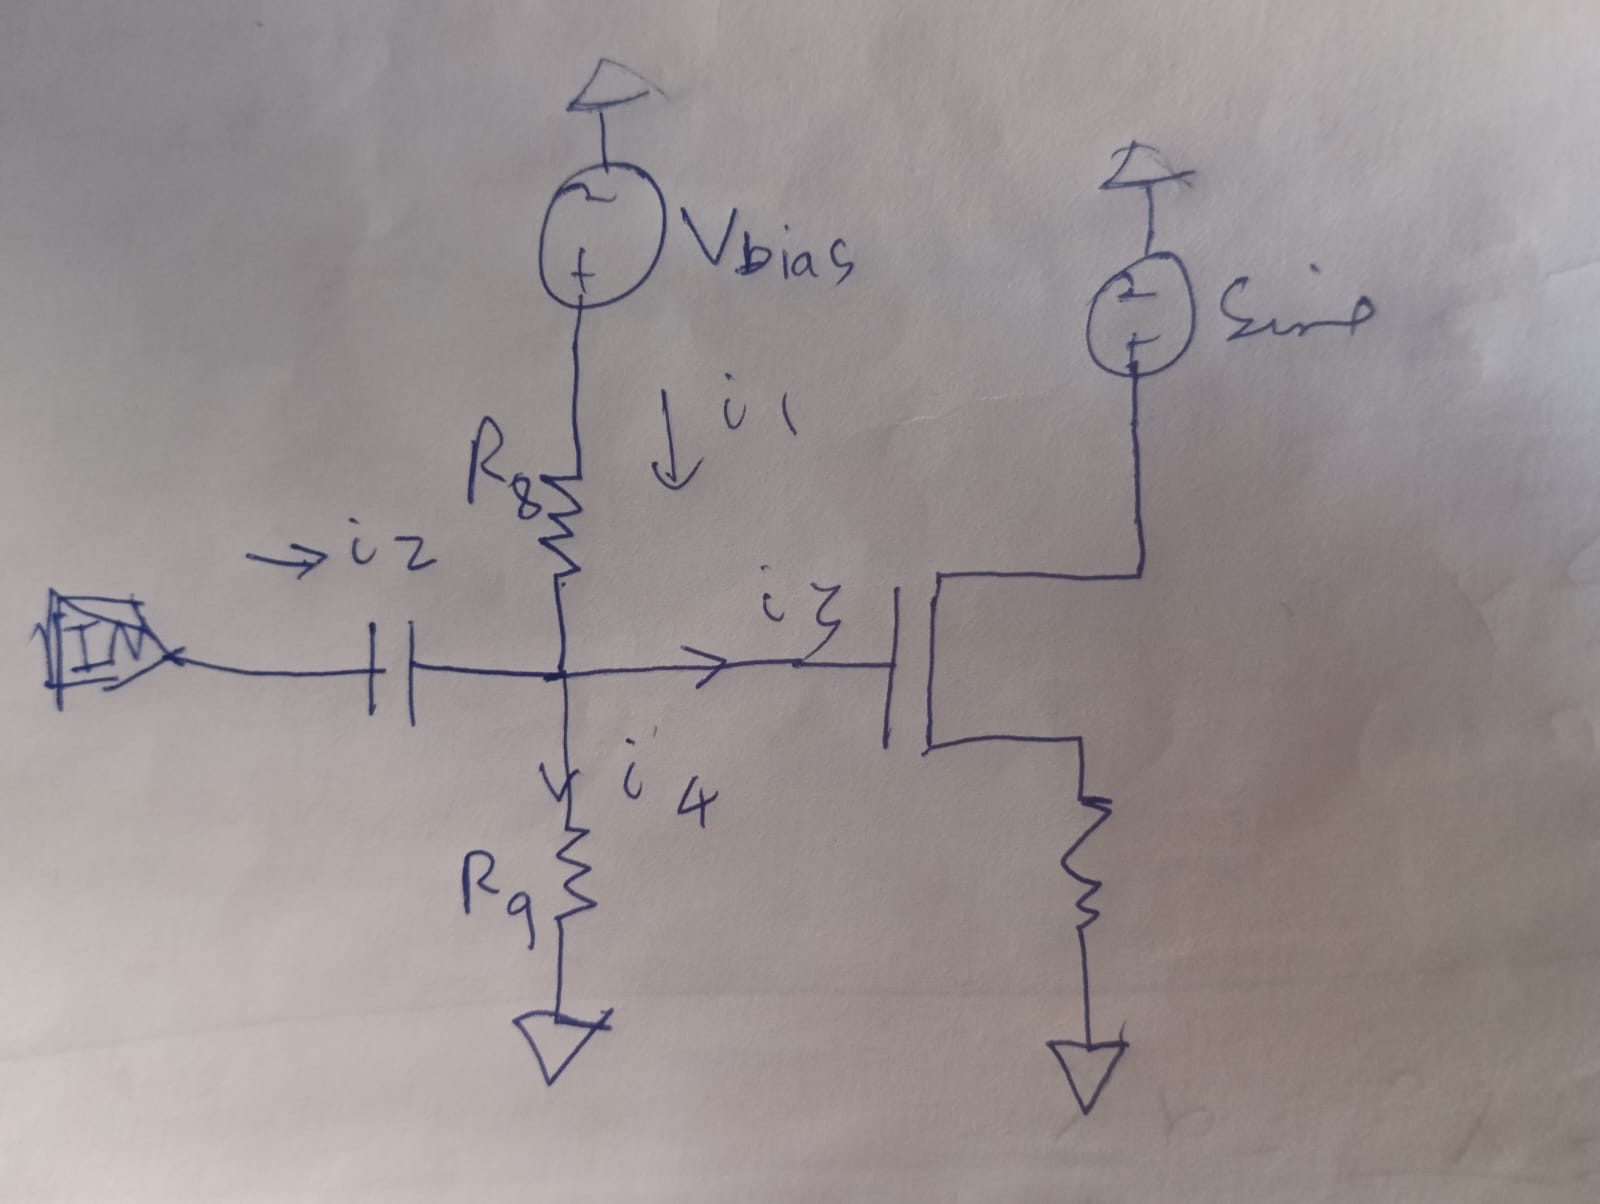
\includegraphics[width=0.85\linewidth]{Images/Mixer_Bias_Calculation.png}
    \caption{Mixer DC Bias Calculation}
    % \label{fig:enter-label}`'
\end{figure}

Applying Kirchoff's current law, we can say that $i_2 +i_1 = i_3 + i_4$. But as there is a capacitor blocking the path of $i_2$ and there will be no flow of current into the gate of the MOSFET. Hence, $i_3 = 0$. This gives us, $i_1 = i_4$. Now, we want the voltage divider formed by $R_8 and R_9$ to give 720 mV ($V_{th}$ of our MOSFET) as the voltage output across $R_9$. Choosing $R_8 = 770k$ (using a high value to reduce current draw), we can calculate $R_9$ as:
$$R_9 = \frac{V_{out} \cdot R_8}{V_{in} - V_{out}}$$
$$R_9 = \frac{0.720 \times 770000}{10 - 0.720}$$
$$R_9 \approx 60k$$


\subsection{Demodulator}
The demodulator circuit is designed to recover the original message signal from the modulated DSB-SC signal. The demodulation process involves multiplying the received DSB-SC signal with a local oscillator (LO) signal that is coherent with the carrier frequency of the received signal. This multiplication process effectively shifts the frequency components of the modulated signal down to baseband, allowing for easy extraction of the original message signal.

This multiplication is done using a switching mode demodulator, similar to the modulator circuit. The output of the demodulator is then passed through a low-pass filter (LPF) to remove the high-frequency components and recover the original message signal.

\begin{figure}
    \centering
    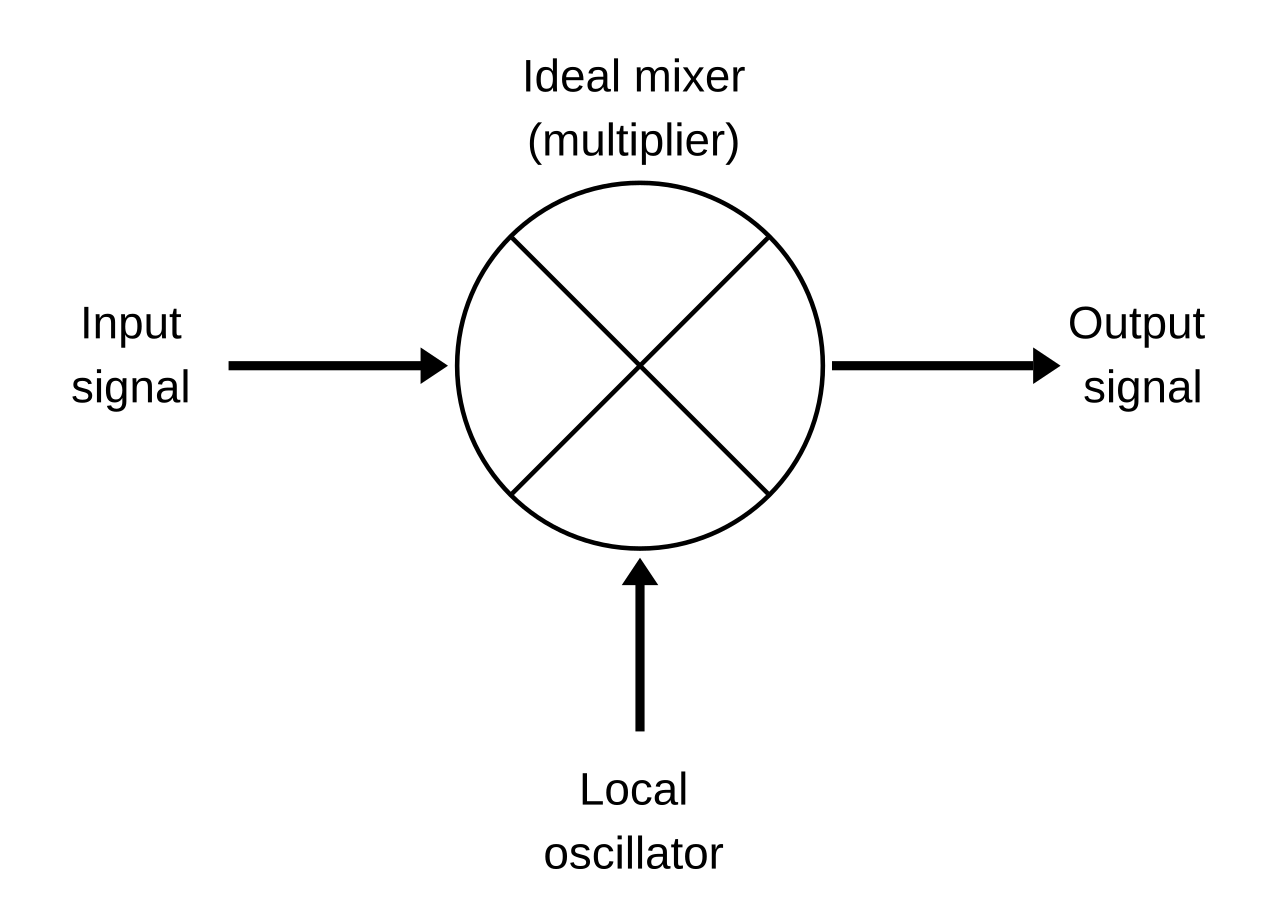
\includegraphics[width=0.5\linewidth]{mixer.png}
    \caption{Mixer}
    % \label{fig:enter-label}
\end{figure}

The output of the multiplier is then passed through a low-pass filter (LPF) to remove the high-frequency components and recover the original message signal. The LPF is designed to have a cutoff frequency that allows the baseband message signal to pass through while attenuating the higher frequency components.

\begin{figure}
    \centering
    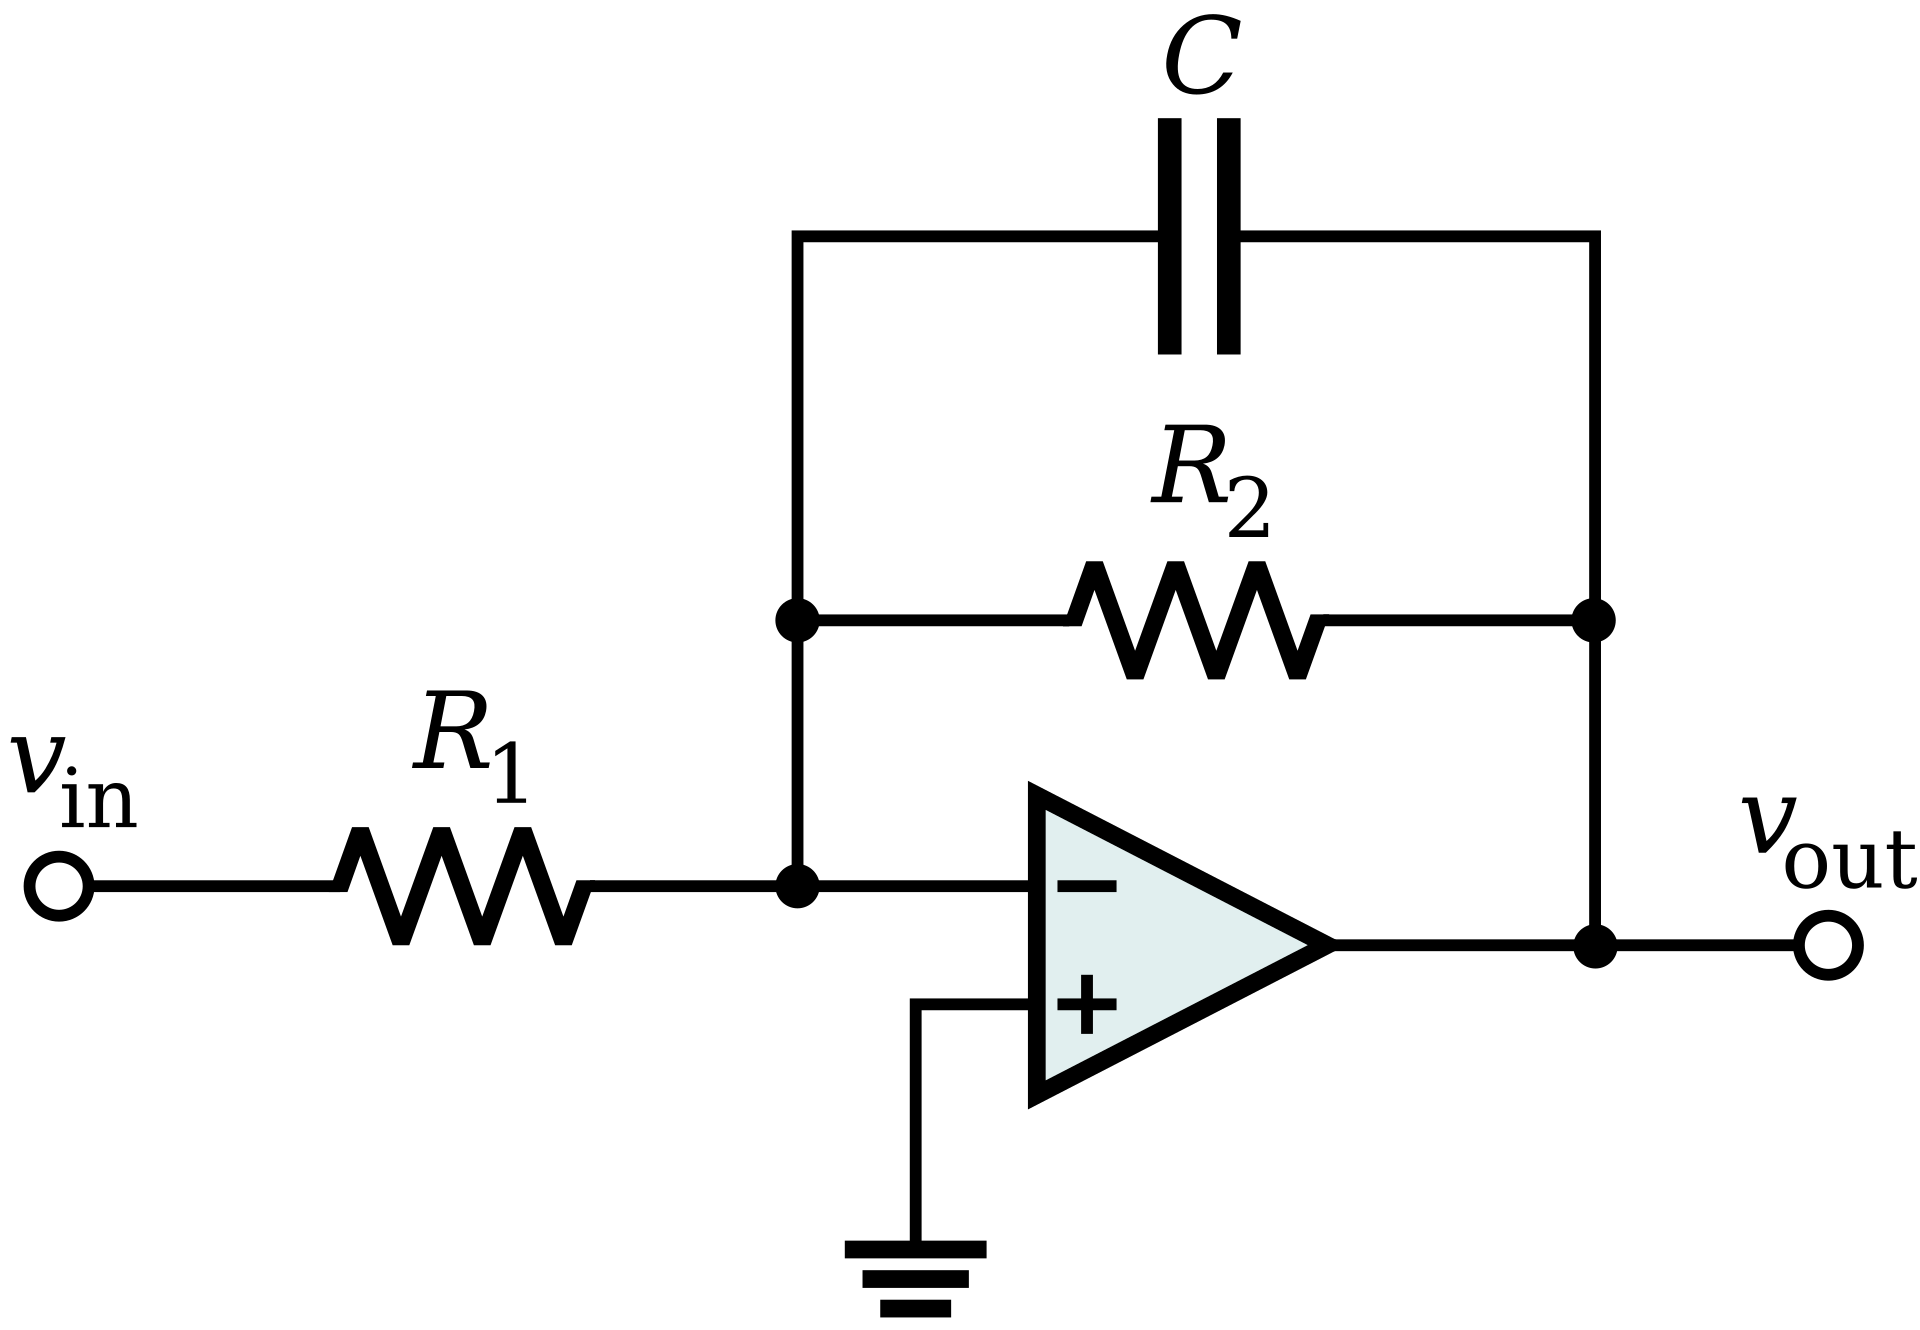
\includegraphics[width=0.75\linewidth]{Images/Active_LPF.png}
    \caption{Active Low Pass Filter}
\end{figure}

The output of the LPF is the recovered message signal, which should closely resemble the original message signal before modulation. The performance of the demodulator circuit is evaluated by comparing the recovered message signal with the original message signal.

\section{Experimental Setup \& Methodology}
\subsection{LTSpice Simulation}
The circuit was designed and simulated using LTSpice. The simulation allowed us to analyze the performance of the modulator and demodulator circuits, as well as the local oscillator. The results obtained from the simulations were compared with the experimental results to validate the design.

The full circuit designed in LTSpice with \textbf{intial calculations}.
\begin{figure}
    \centering
    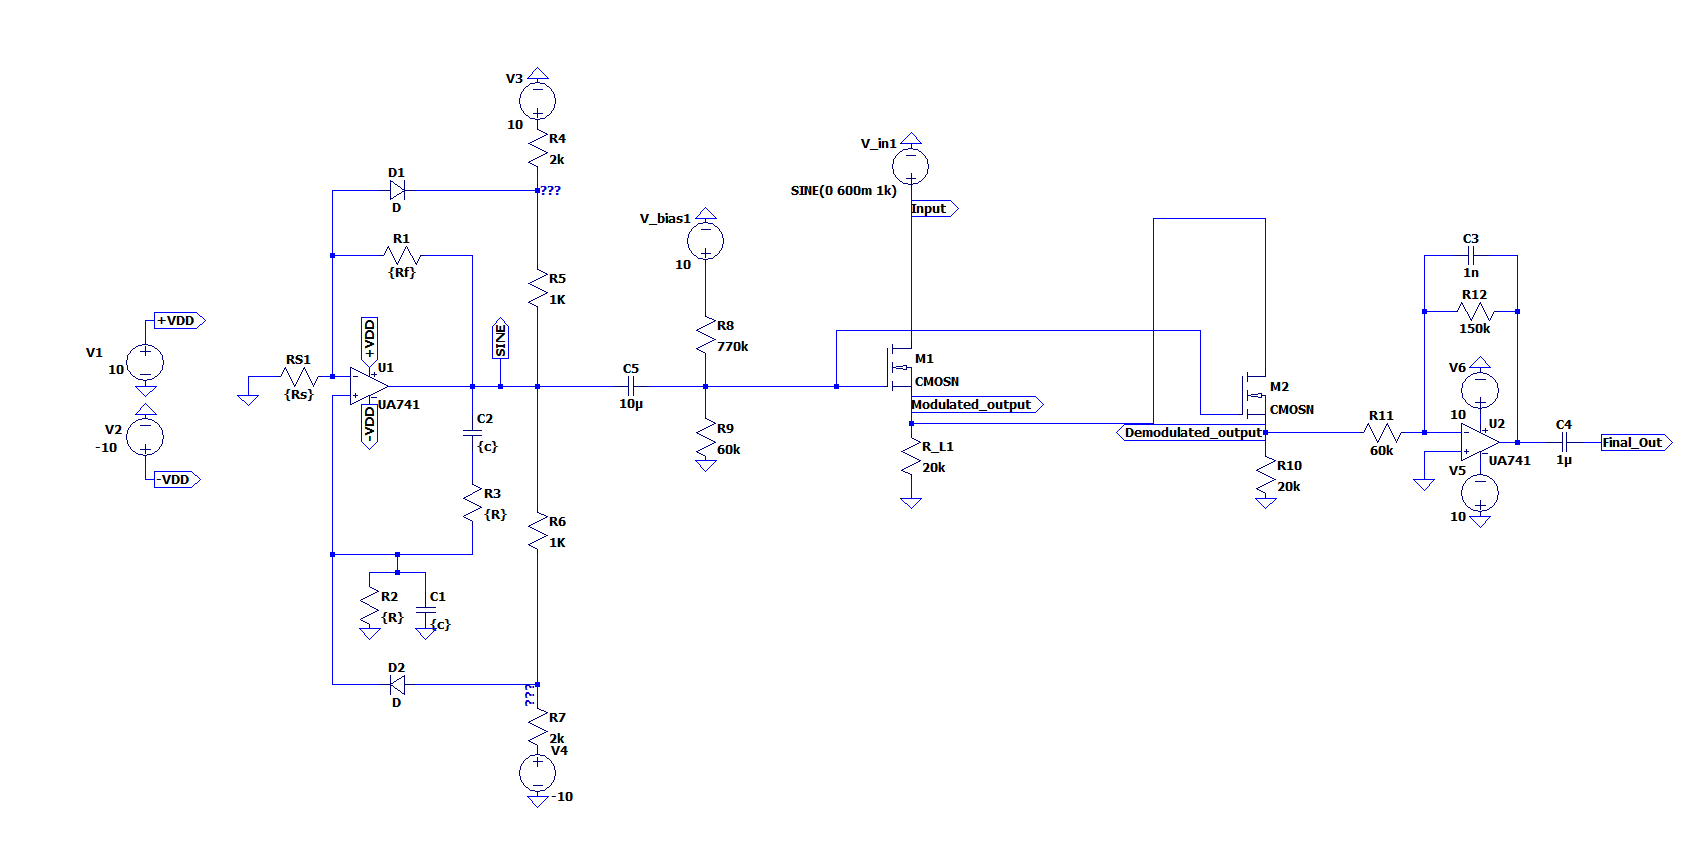
\includegraphics[width=1\linewidth]{Images/Full_circuit_ltspice.png}
    \caption{LTSpice Simulation of the Full Circuit}
    % \label{fig:enter-label}
\end{figure}
Final Output of the circuit in LTSpice:
\begin{figure}
    \centering
    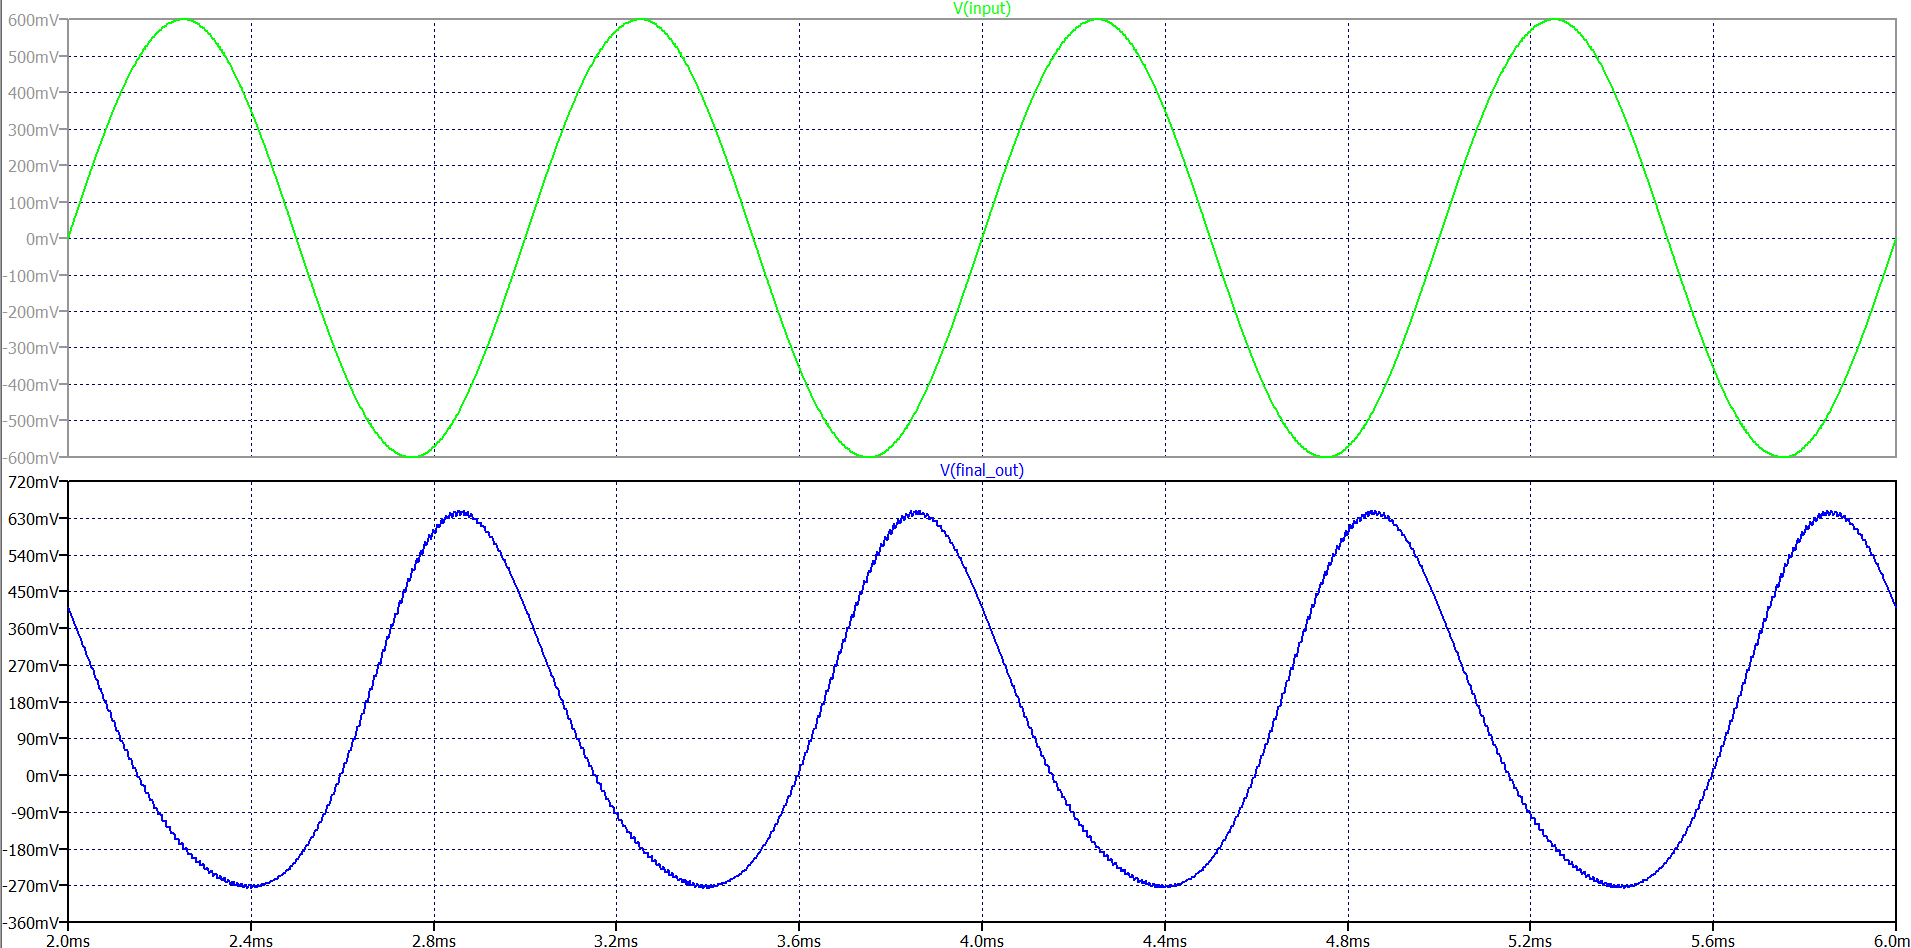
\includegraphics[width=1\linewidth]{Images/final_out_ltspice.png}
    \caption{Message and retrieved message signal (Simulation)}
    % \label{fig:enter-label}
\end{figure}

Individual Stages in LTSpice $ \& $ their outputs:
\subsubsection{Oscillator:}
\begin{figure}
    \centering
    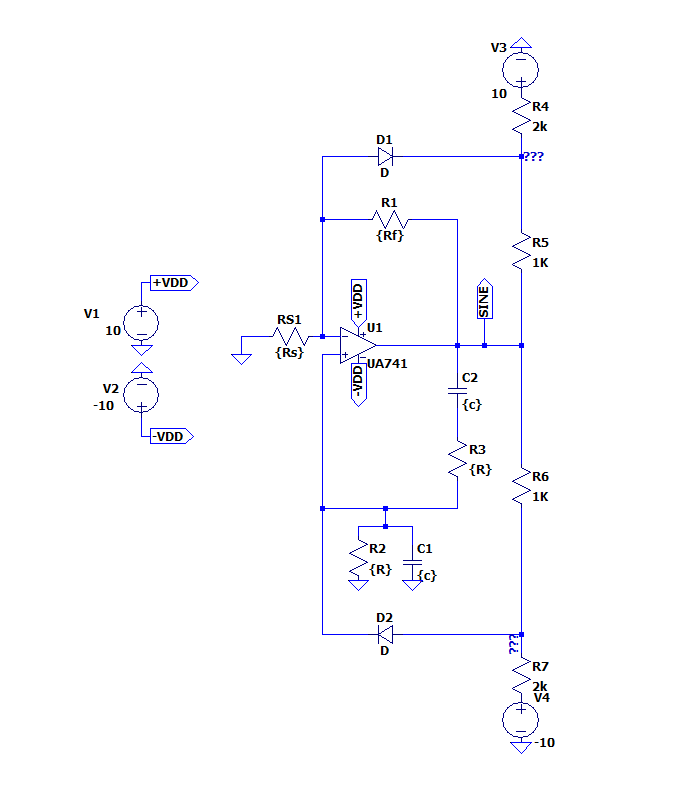
\includegraphics[width=1\linewidth]{Images/Wein_bridge_oscillator_ltspice.png}
    \caption{Circuit of the Local Oscillator (Simulation)}
    % \label{fig:enter-label}
\end{figure}

\begin{figure}
    \centering
    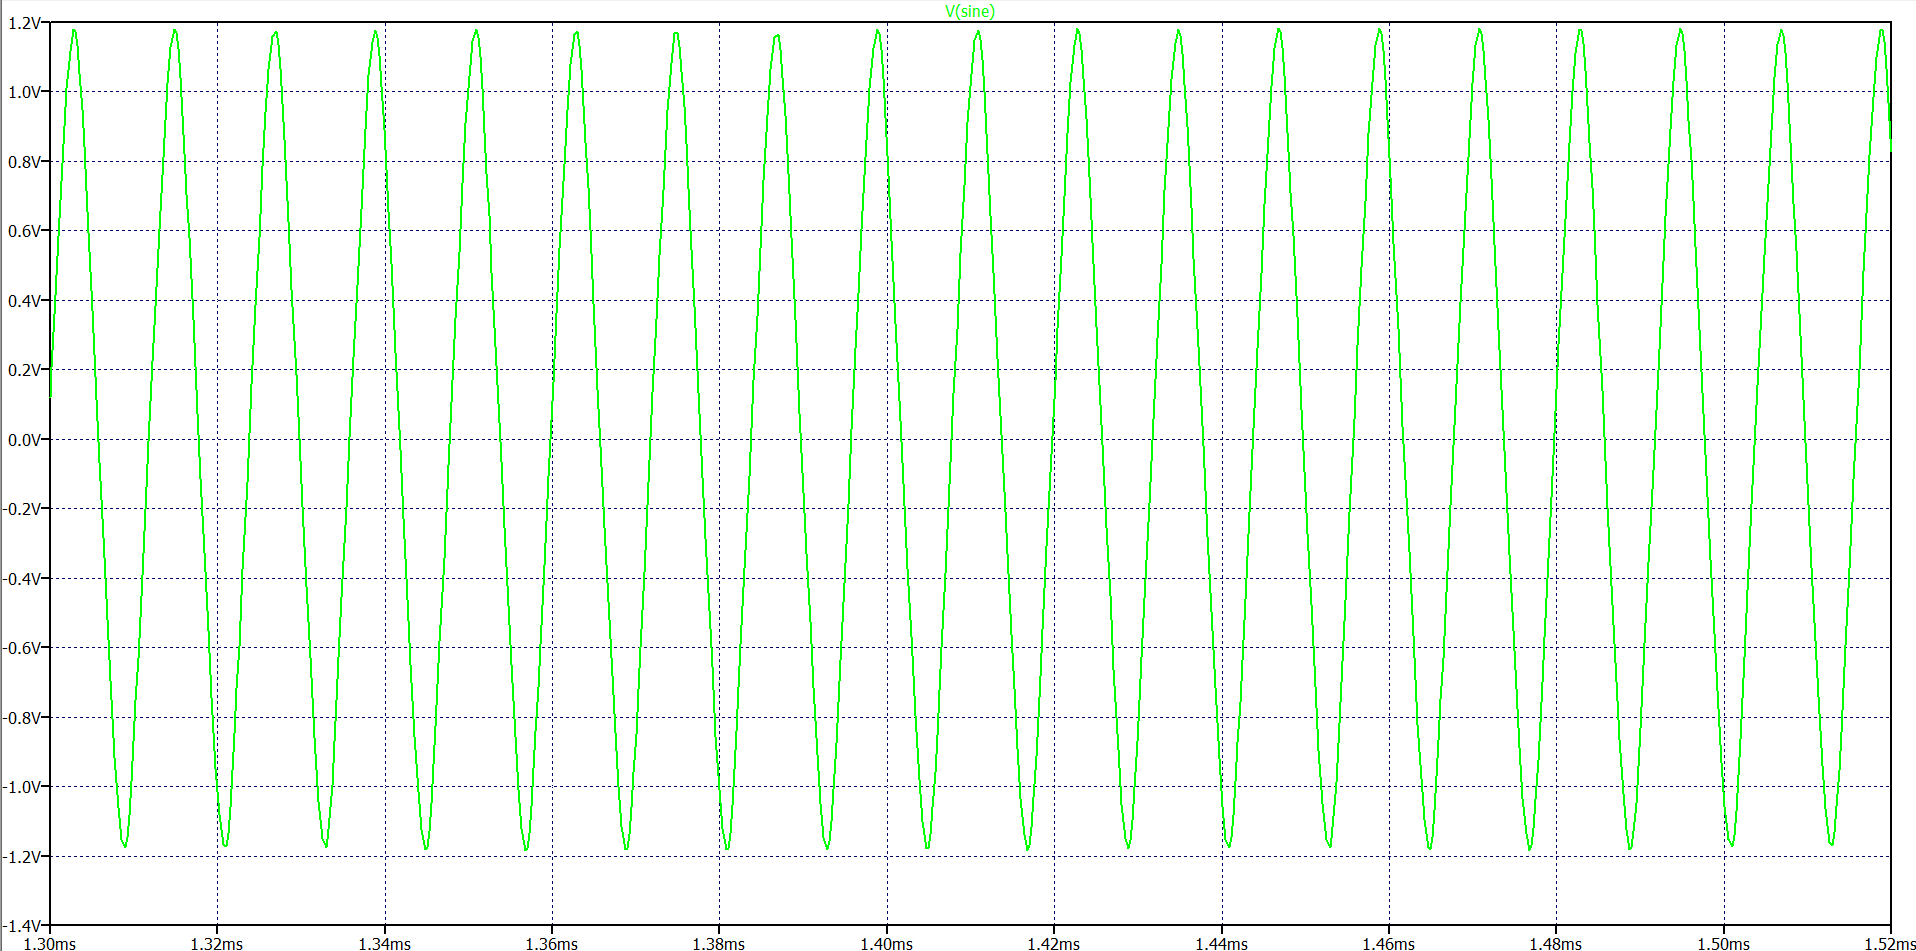
\includegraphics[width=1\linewidth]{Images/Osc_simulation.png}
    \caption{Simulation output of the Oscillator}
    % \label{fig:enter-label}
\end{figure}

The fft of the output of the oscillator is shown below:
\begin{figure}
    \centering
    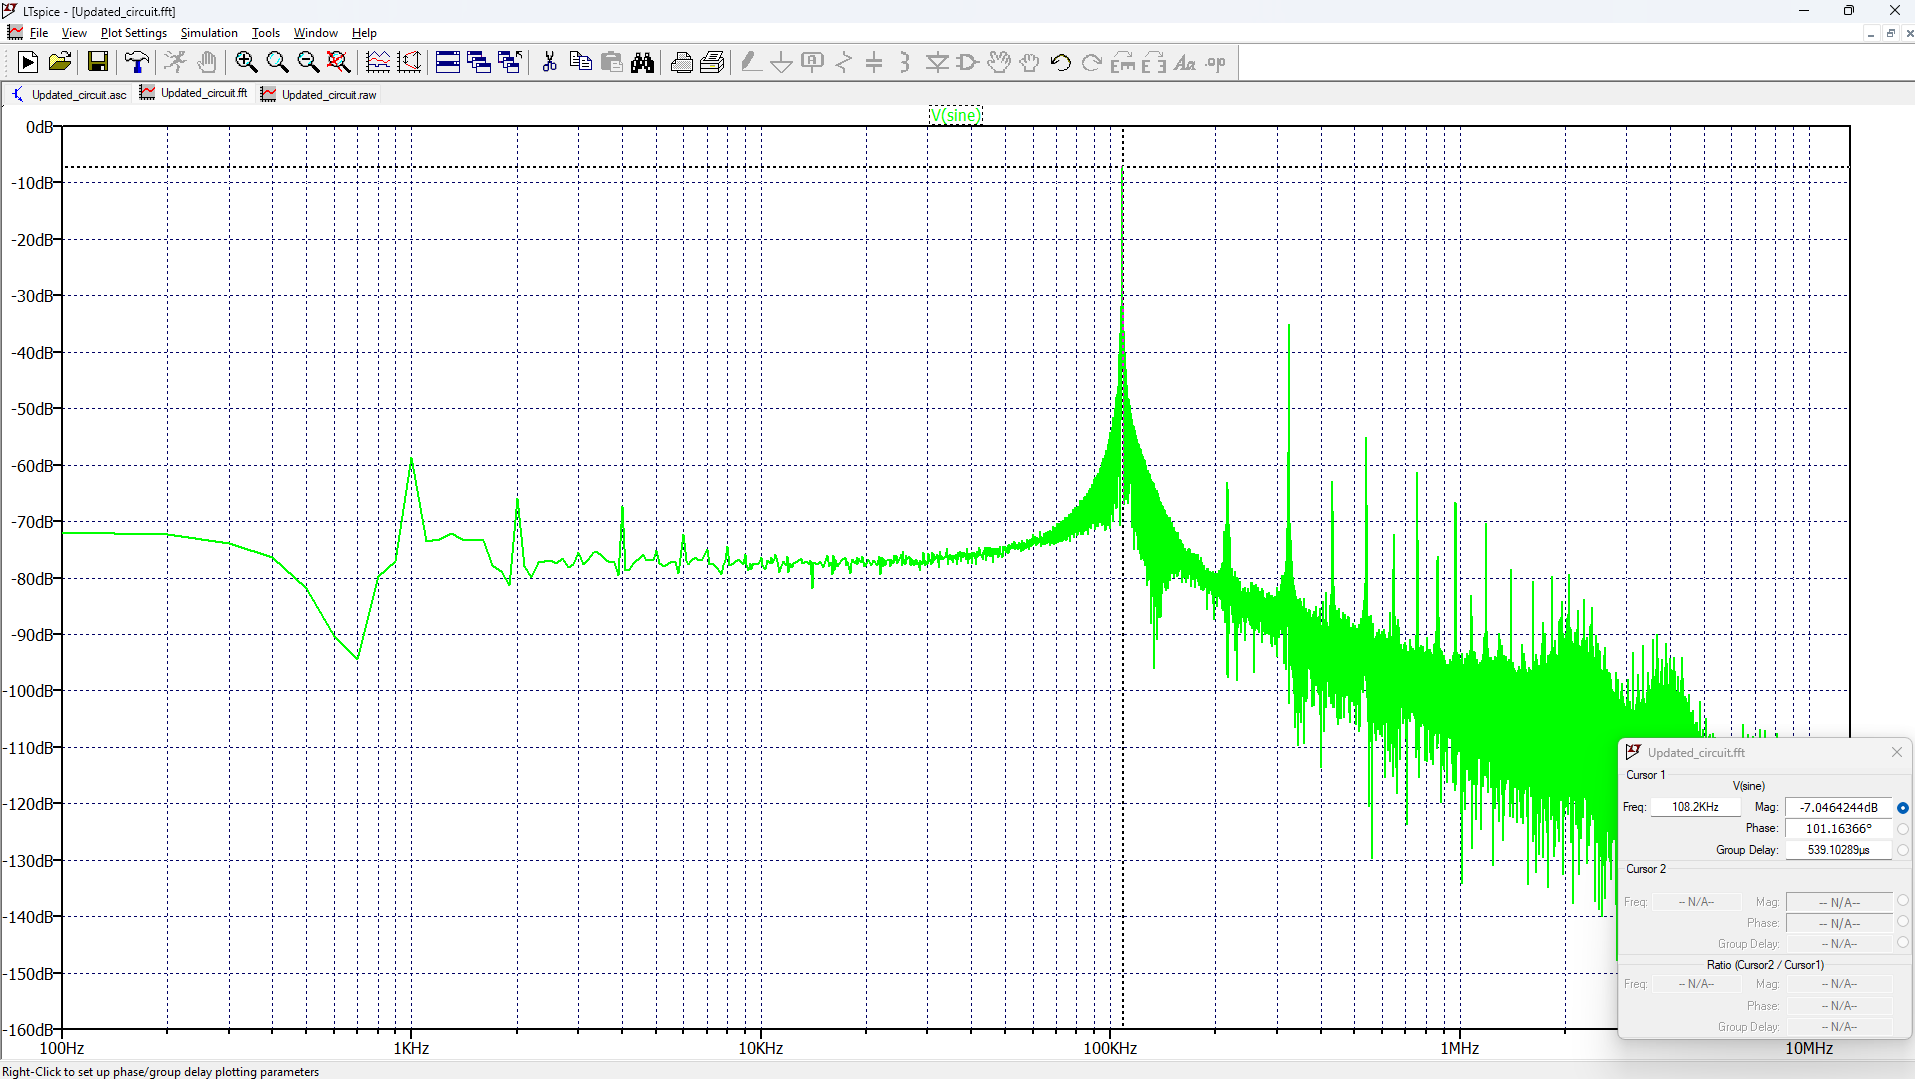
\includegraphics[width=1\linewidth]{Images/fft_sine_osc.png}
    \caption{FFT of the output of the oscillator (Simulation)}
    % \label{fig:enter-label}
\end{figure}
The output of the oscillator is a sine wave with a frequency of 108 kHz. The FFT of the output shows a peak at the carrier frequency, indicating that the oscillator is generating the desired carrier signal.

\subsubsection{Modulator :}
The modulator circuit is designed to modulate the message signal with the carrier signal generated by the local oscillator. The circuit uses a MOSFET as a switch to perform the modulation. The output of the modulator is a DSB-SC signal.

\begin{figure}
    \centering
    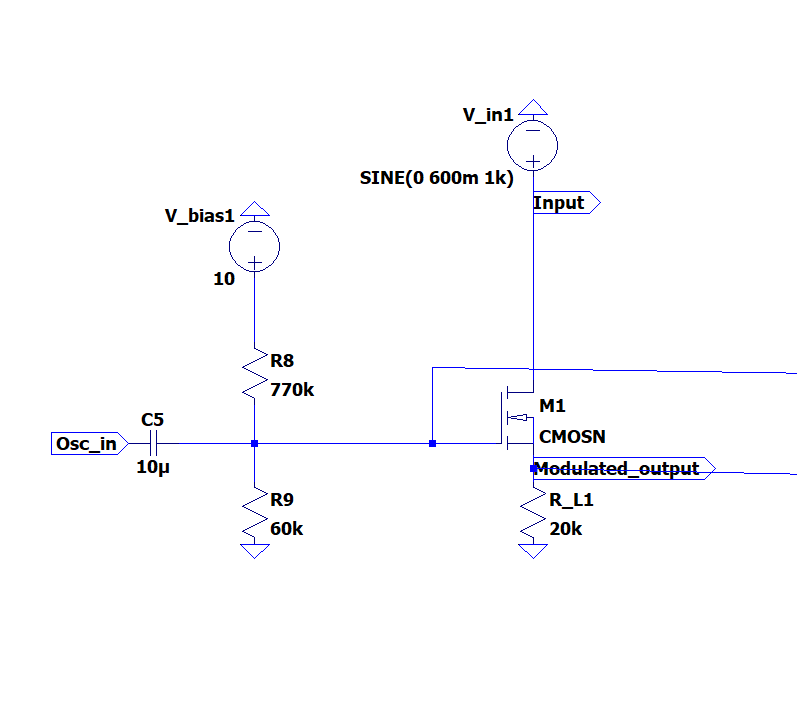
\includegraphics[width=1\linewidth]{Images/Modulator_ltspice.png}
    \caption{Circuit diagram of the modulator}
    % \label{fig:enter-label}
\end{figure}
\begin{figure}
    \centering
    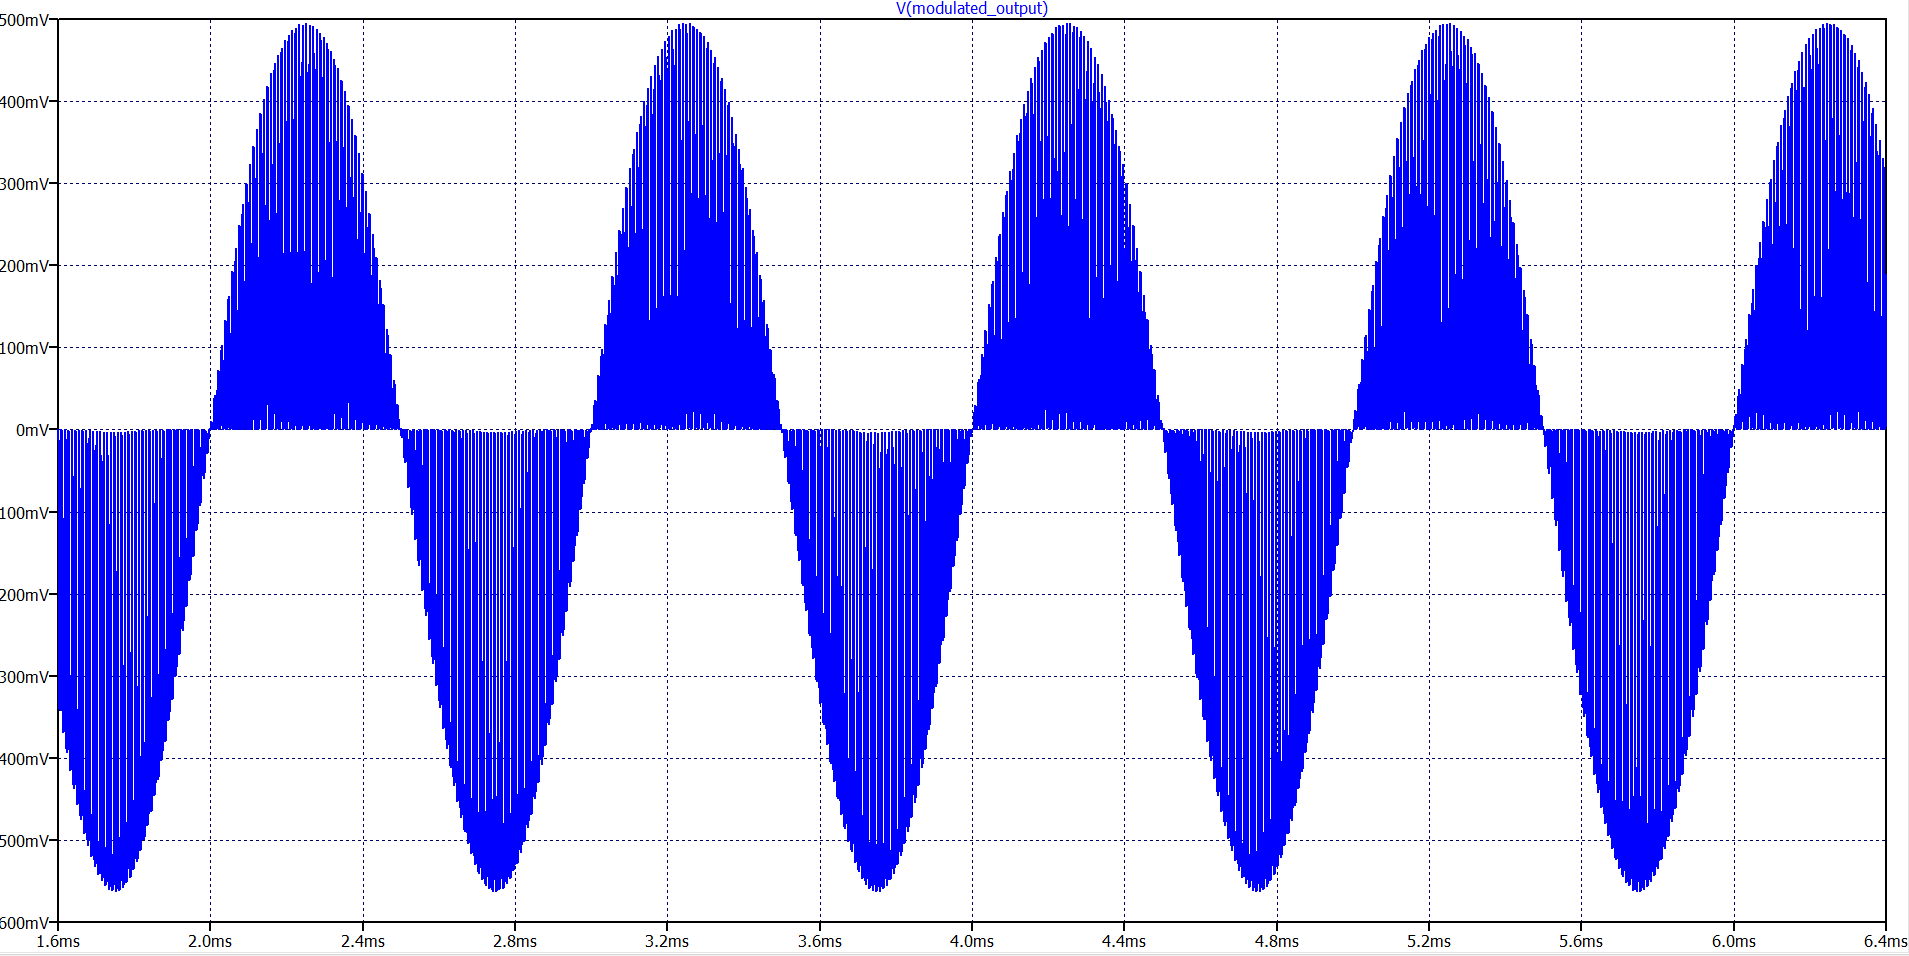
\includegraphics[width=1\linewidth]{Images/modulated_output_ltspice.png}
    \caption{Output of the modulator circuit (Simulation)}
    % \label{fig:enter-label}
\end{figure}

\subsubsection{Demodulator:}
\begin{figure}
    \centering
    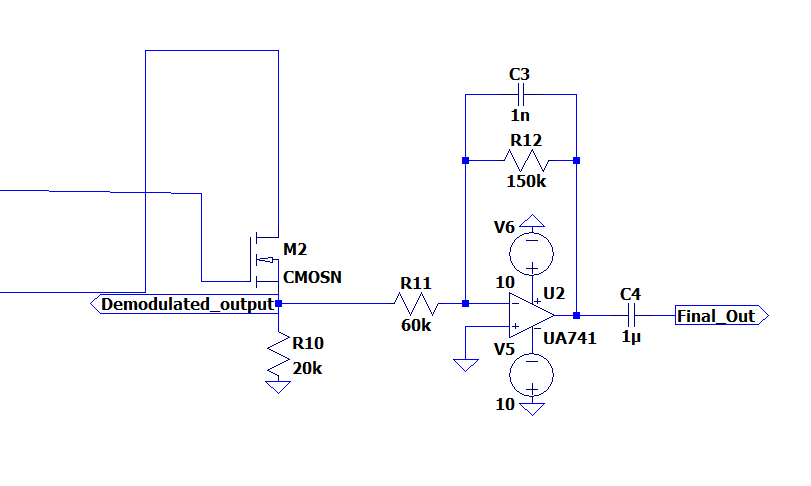
\includegraphics[width=1\linewidth]{Images/Demodulator_ltspice.png}
    \caption{Circuit diagram of the demodulator}
    % \label{fig:enter-label}
\end{figure}

\begin{figure}
    \centering
    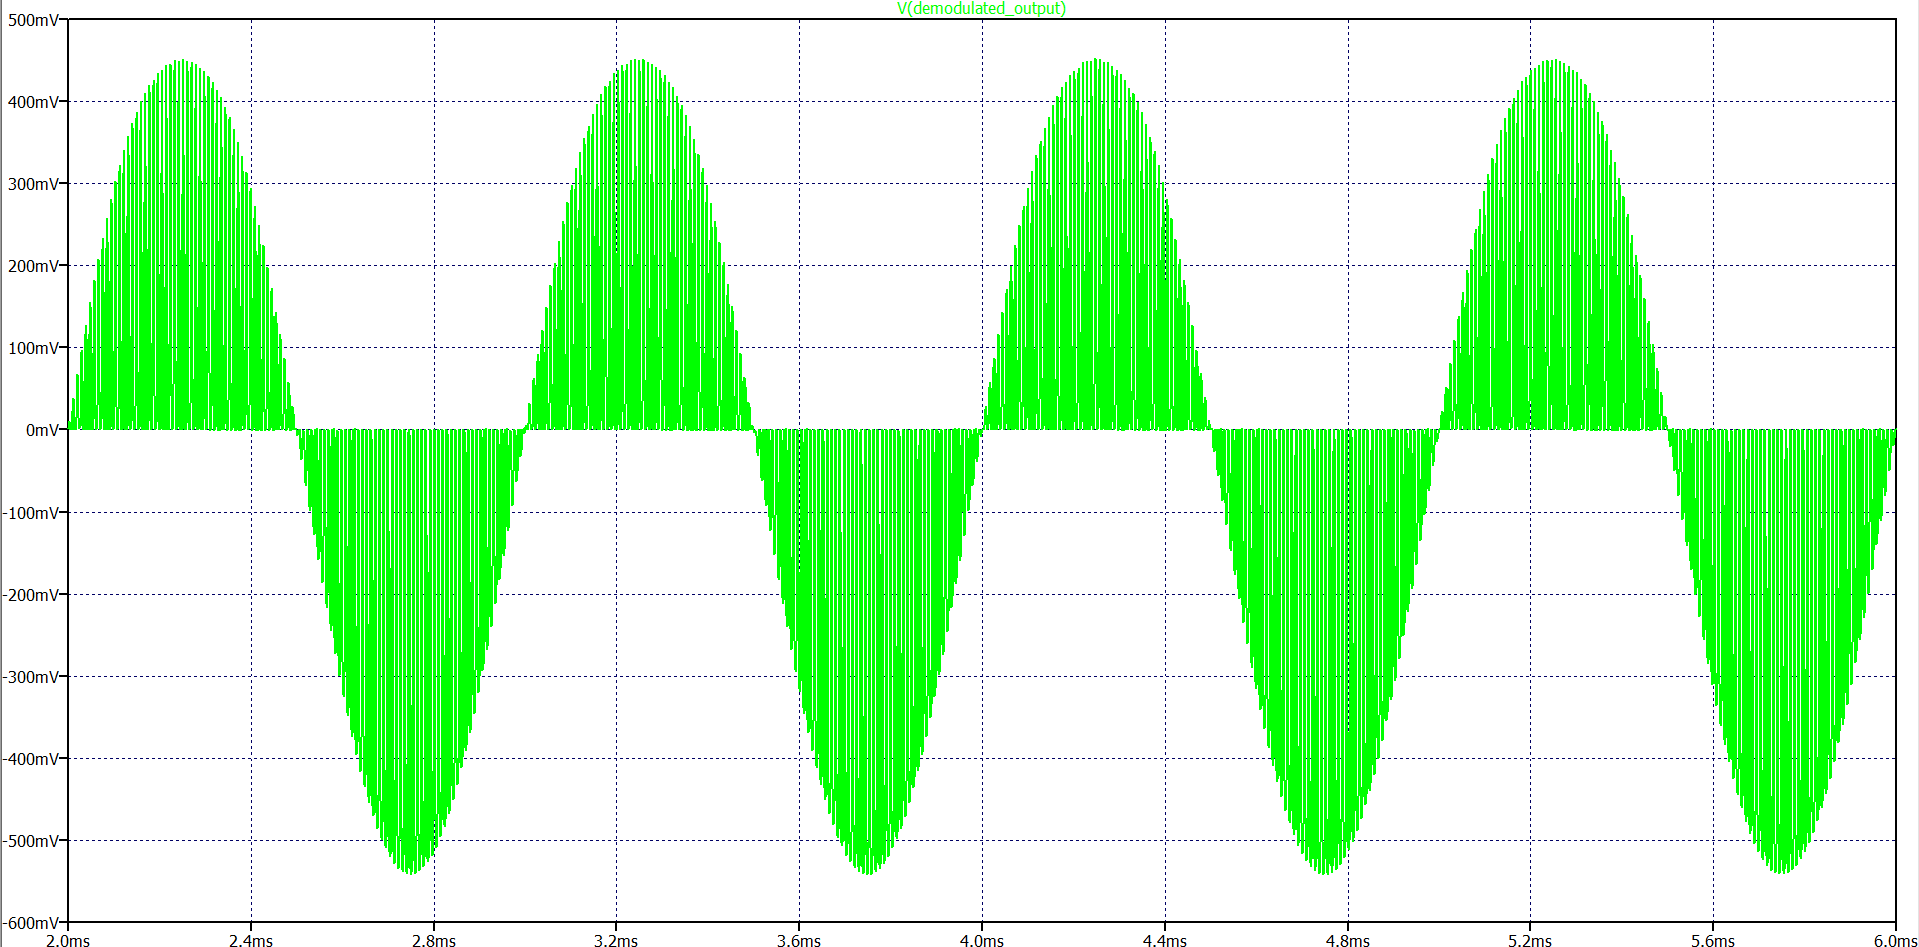
\includegraphics[width=1\linewidth]{Images/demodulated_output_ltspice.png}
    \caption{Output of the demodulator circuit (Simulation)}
    % \label{fig:enter-label}
\end{figure}


\subsection{Hardware Implementation}
The hardware implementation of the circuit was done using a breadboard and various electronic components. The components used in the circuit include resistors, capacitors, MOSFETs, and operational amplifiers. The circuit was powered using a DC power supply, and the output signals were observed using an oscilloscope.
The circuit was built in a modular fashion, with each stage (oscillator, modulator, and demodulator) being tested individually before integrating them into the complete system. The performance of the circuit was evaluated by observing the output waveforms at various points in the circuit using an oscilloscope.

\begin{figure}
    \centering
    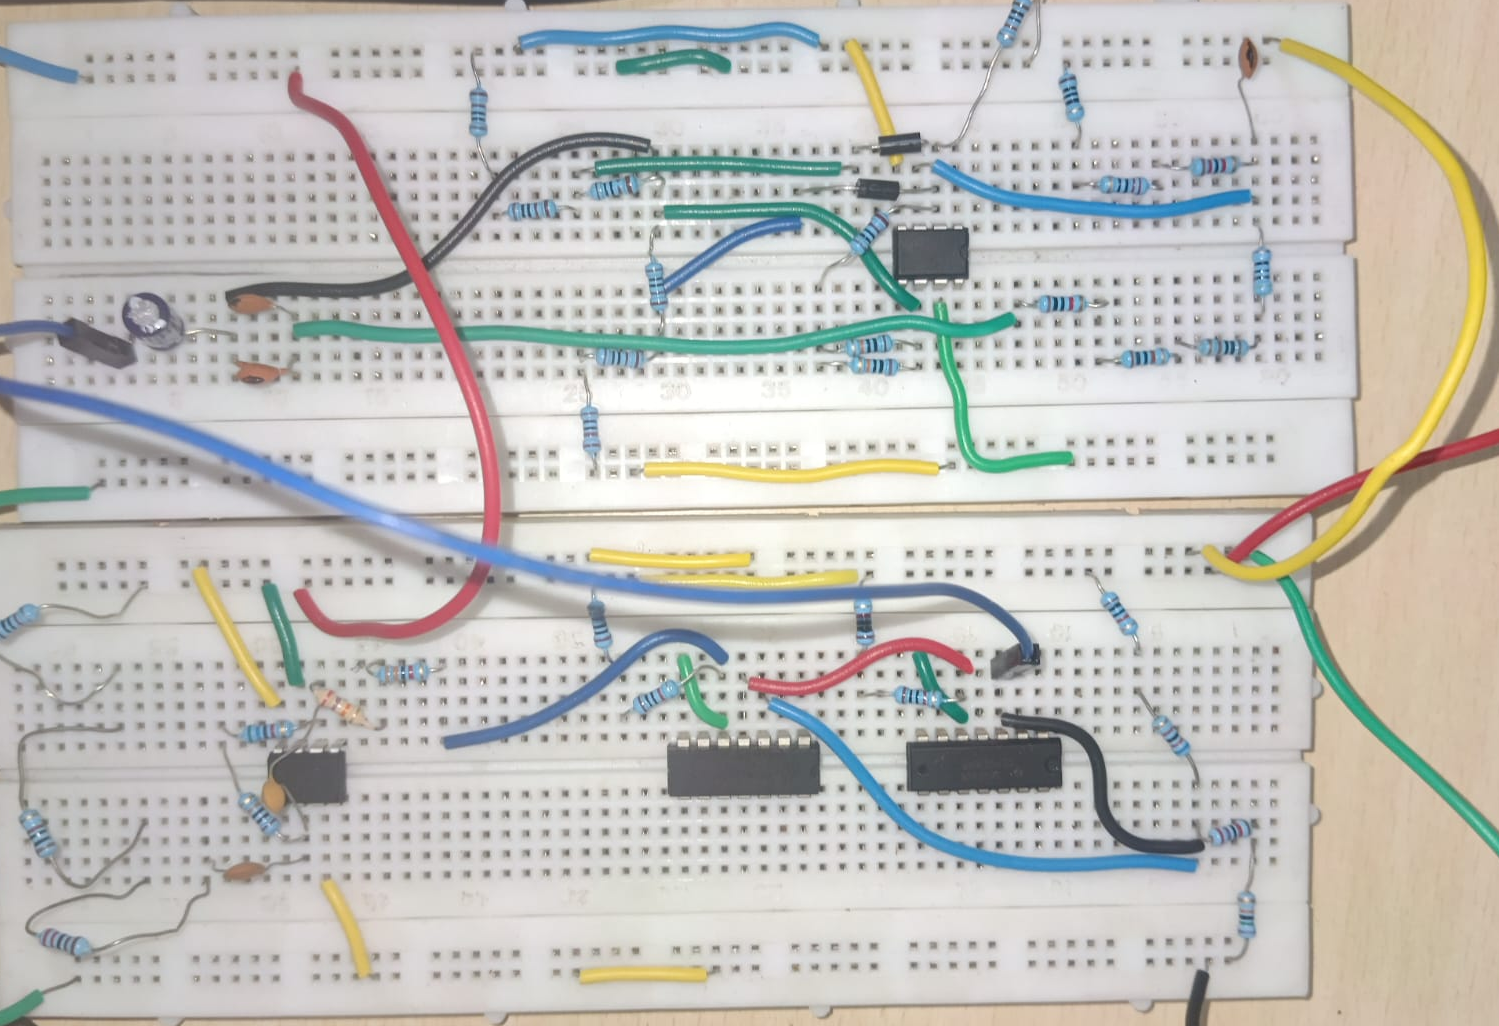
\includegraphics[width=1\linewidth]{Images/Full_circuit_hardware.png}
    \caption{Image of the hardware implementation of the circuit}
    % \label{fig:enter-label}
\end{figure}

Final output from the hardware implementation:
\begin{figure}
    \centering
    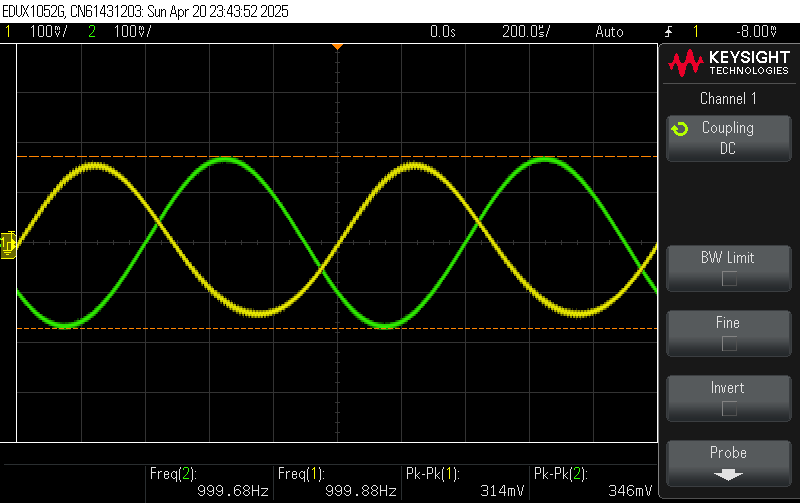
\includegraphics[width=1\linewidth]{Images/final_out_circuit.png}
    \caption{Input message signal and retrieved message signal (Hardware)}
    % \label{fig:enter-label}
\end{figure}
\subsubsection{Local Oscillator:}
\begin{figure}
    \centering
    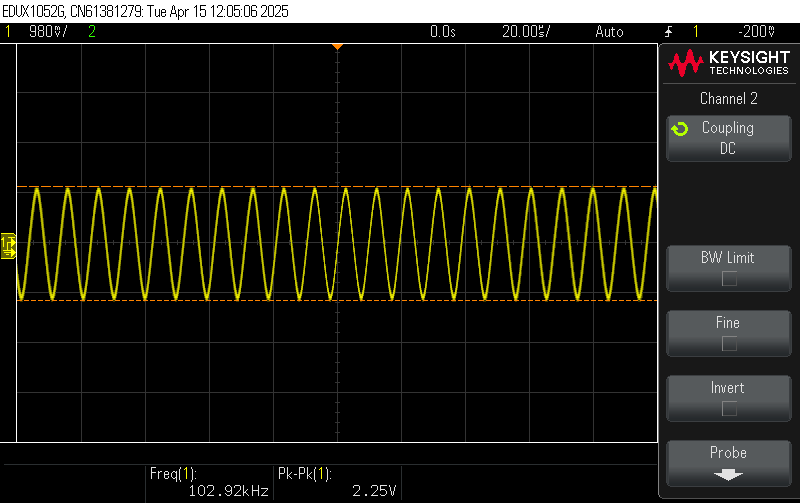
\includegraphics[width=1\linewidth]{Images/osc_circuit_out.png}
    \caption{Output of the oscillator (Hardware)}
    % \label{fig:enter-label}
\end{figure}
We were able to get a sine wave of 108 kHz from the oscillator circuit. The output was observed using an oscilloscope. The output of the oscillator is a sine wave with a frequency of 108 kHz. The FFT of the output shows a peak at the carrier frequency, indicating that the oscillator is generating the desired carrier signal.

\begin{figure}
    \centering
    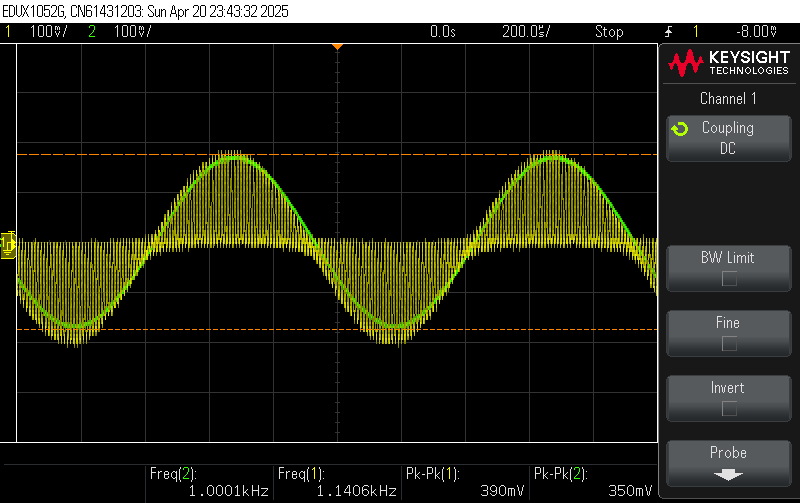
\includegraphics[width=1\linewidth]{Images/modulated_out_circuit.png}
    \caption{Modulated output of the modulator circuit (Hardware)}
    % \label{fig:enter-label}
\end{figure}

\begin{figure}
    \centering
    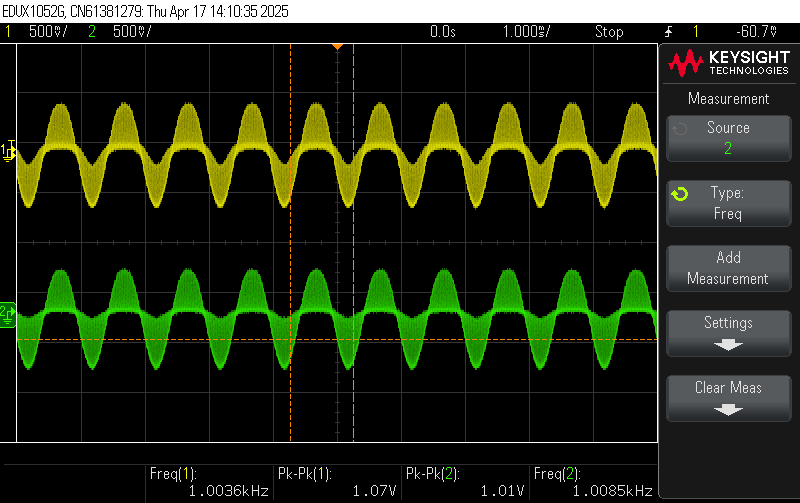
\includegraphics[width=1\linewidth]{Images/modulated_demodulated.png}
    \caption{Modulated and demodulated Output (Hardware)}
    % \label{fig:enter-label}
\end{figure}

\begin{figure}
    \centering
    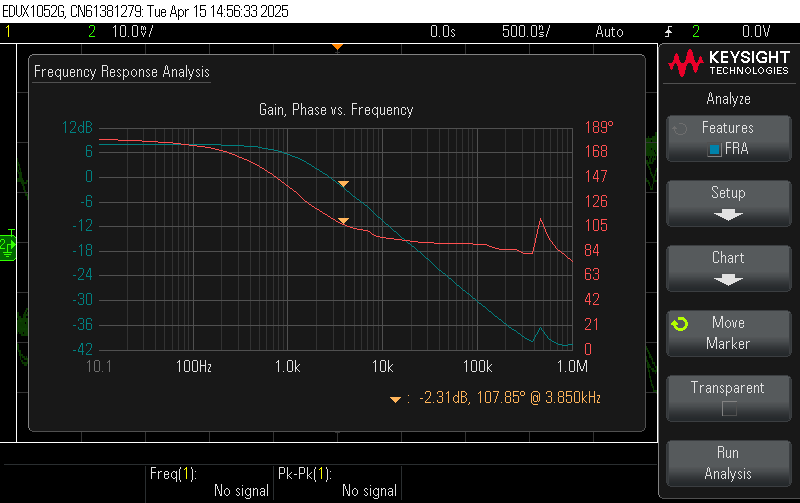
\includegraphics[width=1\linewidth]{Images/filter_response.png}
    \caption{Bode plot of the filter circuit (Hardware)}
    % \label{fig:enter-label}
\end{figure}

\begin{figure}
    \centering
    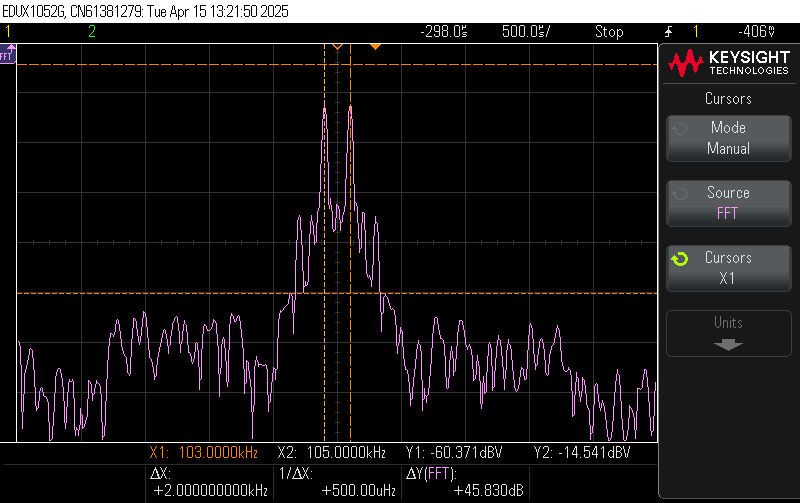
\includegraphics[width=1\linewidth]{Images/modulated_output_fft.png}
    \caption{FFT of the modulated output (Hardware)}
    % \label{fig:enter-label}
\end{figure}

\begin{figure}
    \centering
    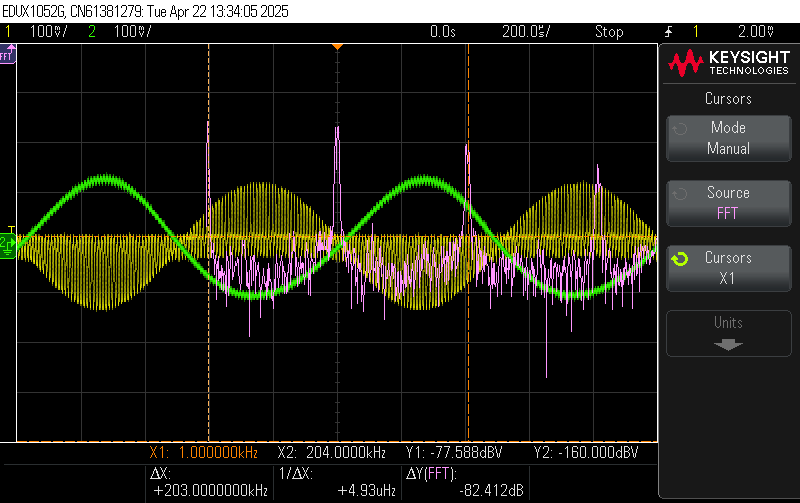
\includegraphics[width=1\linewidth]{Images/demodulated_output_fft.png}
    \caption{FFT of the demodulated output (Hardware)}
    % \label{fig:enter-label}
\end{figure}

\begin{figure}
    \centering
    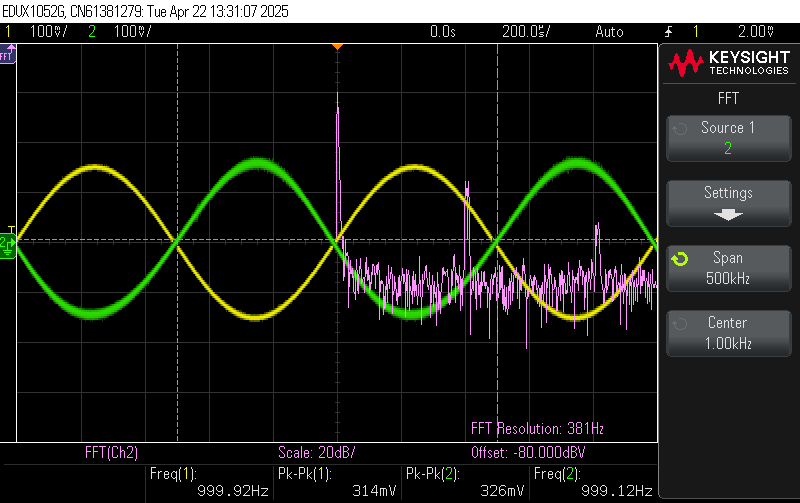
\includegraphics[width=1\linewidth]{Images/recovered_message_fft.png}
    \caption{FFT of the recovered message signal (Hardware)}
    % \label{fig:enter-label}
\end{figure}

\section{Conclusion}
The project successfully demonstrated the design, implementation, and analysis of a Double Sideband Suppressed Carrier (DSB-SC) Amplitude Modulation (AM) modulator and demodulator circuit prototype. The experimental results confirmed the effectiveness of the DSB-SC technique in modulating and demodulating signals, showcasing its potential for efficient communication systems.The project also highlighted the importance of coherent detection and the challenges associated with phase synchronization in demodulation.

Github: \href{https://github.com/MadhanSaiKrishna/AM-Modulator-Demodulator}{Repository Link}

Youtube: \href{https://youtu.be/ZRsL6npqL7Y}{Video Link}




\begin{thebibliography}{00}
\bibitem{wiki-dsb}
\textit{Double-sideband suppressed-carrier transmission: }
\href{https://en.wikipedia.org/wiki/Double-sideband_suppressed-carrier_transmission}{Link}
\bibitem{wiki-AM}
\textit{Amplitude Modulation}
\href{https://en.wikipedia.org/wiki/Amplitude_modulation}{Link}
\bibitem{Text-book-Madhow}
\textit{"Introduction to Communication Systems" by Upamanyu Madhow}
\bibitem{Text-book-BPLathi}
\textit{"MODERN DIGITAL AND ANALOG COMMUNICATION SYSTEMS" by B.P. Lathi}
\bibitem{Text-book-Razavi}
\textit{"RF Microelectronics" by Behazad Razavi}
\bibitem{RC-Phase-Shift}
\href{https://vesit.ves.ac.in/RC_phase_shift/theory}{\textit{Phase Shiftor Circuit}}
\bibitem{RC-Calculator}
\href{https://www.omnicalculator.com/physics/rc-circuit}{RC Resonant frequency calculator}
\bibitem{FET_Mixer}
\href{https://www.electronics-notes.com/articles/radio/rf-mixer/fet-rf-mixer.php}{FET based RF Mixer}
\bibitem{Active LPF}
\href{https://www.electronics-tutorials.ws/filter/filter_5.html}{Active Low Pass Filter}
\bibitem{Active Low Pass Filter}
\href{https://en.wikipedia.org/wiki/Low-pass_filter}{Active Low Pass Filter - Wikipedia}
\bibitem{Phase Shifter Circuit}
\href{https://wiraelectrical.com/phase-shifter-formula-and-operation/}{Phase Shifter Circuit}
\bibitem{wiki-Barkhausen-Criterion}
\href{https://en.wikipedia.org/wiki/Barkhausen_stability_criterion}{Barkhausen stability criterion}
\end{thebibliography}
% \vspace{12pt}
% \color{red}
% IEEE conference templates contain guidance text for composing and formatting conference papers. Please ensure that all template text is removed from your conference paper prior to submission to the conference. Failure to remove the template text from your paper may result in your paper not being published.

\end{document}
